\documentclass[10pt]{mypackage}

% sans serif font:
%\usepackage{cmbright}
%\usepackage{sfmath}
%\usepackage{bbold} %better blackboard bold

%serif font + different blackboard bold for serif font
\usepackage{newpxtext,eulerpx}
\renewcommand*{\mathbb}[1]{\varmathbb{#1}}
\pagestyle{fancy}
\usetikzlibrary{angles, quotes, intersections}
\usetikzlibrary{bending} % for arrow head angle
%\contourlength{1.0pt}
\usetikzlibrary{3d}

\usepackage[outline]{contour} % glow around text
\tikzset{>=latex} % for LaTeX arrow head

\colorlet{myblue}{blue!65!black}
\colorlet{mydarkblue}{blue!50!black}
\colorlet{myred}{red!65!black}
\colorlet{mydarkred}{red!40!black}
\colorlet{veccol}{green!70!black}
\colorlet{vcol}{green!70!black}
\colorlet{xcol}{blue!85!black}
\colorlet{pcol}{red!60!black}
\colorlet{Lcol}{green!50!black}
%\colorlet{projcol}{xcol!60}
%\colorlet{unitcol}{xcol!60!black!85}
%\colorlet{myred}{red!90!black}
%\colorlet{mypurple}{blue!50!red!80!black!80}
\tikzstyle{vector}=[->,very thick,xcol,line cap=round]
\tikzstyle{xline}=[myblue,very thick]
\tikzstyle{yzp}=[canvas is zy plane at x=0]
\tikzstyle{xzp}=[canvas is xz plane at y=0]
\tikzstyle{xyp}=[canvas is xy plane at z=0]
\def\tick#1#2{\draw[thick] (#1) ++ (#2:0.12) --++ (#2-180:0.24)}
%\def\N{100}
\tikzset{axis/.style={thick,-latex}}
\tikzset{vec/.style={thick,blue}}
\tikzset{univec/.style={thick,red,-latex}}
\tikzstyle{rvec}=[->,xcol,very thick,line cap=round]
\tikzstyle{vvec}=[->,vcol,very thick,line cap=round]
\tikzstyle{pvec}=[->,pcol,very thick,line cap=round]
\tikzstyle{Lvec}=[->,Lcol,very thick,line cap=round]
\tikzstyle{mass}=[line width=0.6,red!30!black,draw=red!30!black, %rounded corners=1,
                  top color=red!40!black!30,bottom color=red!40!black!10,shading angle=30]
%Notation
\usepackage{physics}
\newcommand{\del}{\delta\!}
\fancyhf{}
\rhead{Avinash Iyer}
\lhead{Mathematical Methods of Physics: Class Notes}

\setcounter{secnumdepth}{0}

\begin{document}
\RaggedRight
\tableofcontents
\section{Things You Just Gotta Know}%
\subsection{Coordinate Systems}%
\begin{center}
\tdplotsetmaincoords{60}{110}
\begin{tikzpicture}[scale=3, tdplot_main_coords]
    \coordinate (O) at (0,0,0);
    \draw[thick,->] (0,0,0) -- (1,0,0) node[anchor=north east]{$x$};
    \draw[thick,->] (0,0,0) -- (0,1,0) node[anchor=north west]{$y$};
    \draw[thick,->] (0,0,0) -- (0,0,1) node[anchor=south]{$z$};
    \tdplotsetcoord{P}{1}{30}{60}
    \draw plot [mark=*, mark size=0.2] (P) node [right] {\scriptsize$(x,y,z)$}; 
    \draw[dashed] (O) -- (P);
    \draw[dashed, color=black] (O) -- (Pxy);
    \draw[dashed, color=black] (P) -- (Pxy);
    \draw[dashed, color=black] (P) -- (Pz) node [below left] {$z$};
    \draw[dashed, color=black] (Pxy) -- (Px) node [left] {$x$};
    \draw[dashed, color=black] (Pxy) -- (Py) node [above] {$y$};
\end{tikzpicture}

% Polar Coordinates
\tdplotsetmaincoords{60}{110}
\begin{tikzpicture}[scale=3, tdplot_main_coords]
    \coordinate (O) at (0,0,0);
    \draw[thick,->] (0,0,0) -- (1,0,0) node[anchor=north east]{$x$};
    \draw[thick,->] (0,0,0) -- (0,1,0) node[anchor=north west]{$y$};
    \draw[thick,->] (0,0,0) -- (0,0,1) node[anchor=south]{$z$};
    \tdplotsetcoord{P}{1}{30}{60}
    \draw plot [mark=*, mark size=0.2] (P) node [right] {\scriptsize$(\rho,\phi,z)$};
    \draw[dashed] (O) -- (P);
    \draw[->, thick, color=black] (O) -- (Pxy) node [below right] {$\rho$};
    \draw[dashed, color=black] (P) -- (Pxy);
    \tdplotdrawarc{(O)}{0.2}{0}{60}{anchor=north}{$\phi$}
    \draw[dashed, color=black] (P) -- (Pz) node [below left] {$z$};
\end{tikzpicture}
	
% Spherical Coordinates
\tdplotsetmaincoords{60}{110}
\begin{tikzpicture}[scale=3, tdplot_main_coords]
    \coordinate (O) at (0,0,0);
    \draw[thick,->] (0,0,0) -- (1,0,0) node[anchor=north east]{$x$};
    \draw[thick,->] (0,0,0) -- (0,1,0) node[anchor=north west]{$y$};
    \draw[thick,->] (0,0,0) -- (0,0,1) node[anchor=south]{$z$};
    \tdplotsetcoord{P}{1}{30}{60}
    \draw plot [mark=*, mark size=0.2] (P) node [right] {\scriptsize$(r,\theta,\phi)$};
    \draw[->, thick] (O) -- (P) node [midway, below right] {$r$};
    \draw[dashed, color=black] (O) -- (Pxy);
    \draw[dashed, color=black] (P) -- (Pxy);
    \tdplotdrawarc{(O)}{0.2}{0}{60}{anchor=north}{$\phi$}
    \tdplotsetthetaplanecoords{60}
    \tdplotdrawarc[tdplot_rotated_coords]{(0,0,0)}{0.4}{0}%
        {30}{anchor=south}{$\theta$}
\end{tikzpicture}
\end{center}
We want to focus on vector-valued functions of coordinates.
\begin{align*}
  \vec{V}(\mathbf{r}) &= V_x(x,y)\hat{i} + V_y(x,y)\hat{j}.
\end{align*}
Notice that a vector function uses the coordinate system twice. Once for the function's inputs, once for the vectors themselves.
\subsubsection{Polar Coordinates}%
\begin{center}
  %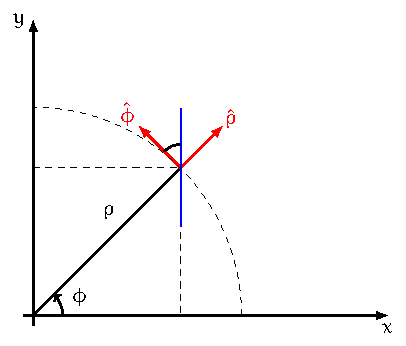
\includegraphics[width=10cm]{polar_coordinates.pdf}
	\begin{tikzpicture}
%		%Grid
%		\draw[thin, dotted] (0,0) grid (8,8);
%		\foreach \i in {1,...,8}
%		{
%			\node at (\i,-2ex) {\i};	
%		}
%		\foreach \i in {1,...,8}
%		{
%			\node at (-2ex,\i) {\i};	
%		}
%		\node at (-2ex,-2ex) {0};
		
		%Coordinates		
		\coordinate (A) at (6,0);
		\coordinate (B) at (0,0);
		\coordinate (C) at (2.5,2.5);
		\coordinate (B') at (2.5,3.5);
		\coordinate (A') at (1.8,3.2);
		
		%Axis
		\draw[thick,-latex] (-1ex,0) -- (6,0) node [below] {$x$};
		\draw[thick,-latex] (0,-1ex) -- (0,5) node [left] {$y$};
		
		%Vectors
		\draw[thick] (0,0) -- (2.5,2.5) node[pos=0.6, above left] {$\rho$};
		\draw[thick, red, -latex] (2.5,2.5) -- (3.2,3.2) node[pos=1.2] {$\hat{\rho}$};
		\draw[thick, red, -latex] (2.5,2.5) -- (1.8,3.2) node[pos=1.3] {$\hat{\phi}$};
		
		%Help Lines
		\draw[dashed] (0,2.5) -- (2.5,2.5) -- (2.5,0);
		\draw[blue, thick] (2.5,3.5) -- (2.5,1.5);
		\draw[dashed] (3.53,0) arc (0:90:3.53);
		
		%Angle
		\pic[draw, ->, thick, "$\phi$", angle eccentricity=1.7] {angle = A--B--C};
		\pic[draw, thick, angle radius=4mm, angle eccentricity=1.7] {angle = B'--C--A'};
		
	\end{tikzpicture}
\end{center}
We can also express the inputs to $ \vec{V} $ in polar coordinates, $(\rho,\phi)$.
\begin{align*}
  \vec{V}(\mathbf{r}) &= V_{\rho}\left(\rho,\phi\right)\hat{i} + V_{\phi}\left(\rho,\phi\right)\hat{j}.
\end{align*}
To extract the input functions, we take
\begin{align*}
  V_x &= \hat{i}\cdot \vec{V}\\
  V_y &= \hat{j}\cdot \vec{V}.
\end{align*}
Alternatively, we can project $ \vec{V} $ onto the $\hat\rho,\hat\phi$ axis:
\begin{align*}
  \vec{V}(\mathbf{r}) &= V_{\rho}\left(\rho,\phi\right)\hat{\rho} + V_{\phi}\left(\rho,\phi\right)\hat{\phi},
\end{align*}
and we extract
\begin{align*}
  V_{\rho} &= \hat{\rho}\cdot \vec{V}\\
  V_{\phi} &= \hat{\phi}\cdot \vec{V}.
\end{align*}
Notice that $\mathbf{r}$ is an abstract vector; we need to project it onto a basis.\newline

For instance, we can take the position vector and project it onto the cartesian and polar axes:
\begin{align*}
  \mathbf{s} &= x\hat{i} + y\hat{j}\\
             &= \rho \cos \phi \hat{i} + \rho \sin \phi \hat{j}\\
             &= \rho \hat{\rho}\\
             &= \sqrt{x^2 + y^2}\hat{\rho}
\end{align*}
The main reason we avoided using the $\hat\rho,\hat\phi$ axis up until this point is that $\rho$ and $\phi$ are \textit{position-dependent}, while the $\hat{i},\hat{j}$ axis is position-independent.\newline

Now, we must figure out the position-dependence of $\hat{\rho}$ and $\hat{\phi}$:
\begin{align*}
  d\mathbf{r} &= \pd{\mathbf{r}}{\rho}d\rho + \pd{\mathbf{r}}{\phi}d\phi.
\end{align*}
If we hold $\phi$ constant, it must be the case that any change in $\rho$ is in the $\hat\rho$ direction. Therefore,
\begin{align*}
  \hat\rho &= \frac{\pd{\mathbf{r}}{\rho}}{\left\Vert \pd{\mathbf{r}}{\rho} \right\Vert}\\
           &= \frac{\cos\phi\hat{i} + \sin\phi\hat{j}}{\left\vert \cos\phi\hat{i} + \sin\phi\hat{j} \right\vert}\\
           &= \cos\phi\hat{i} + \sin\phi\hat{j}.
\end{align*}
Similarly,
\begin{align*}
  \hat\phi &= \frac{\pd{\mathbf{r}}{\phi}}{\norm{\pd{\mathbf{r}}{\rho}}}\\
           &= \frac{-\rho\sin\phi\hat{i} + \rho\cos\phi\hat{j}}{\left\Vert -\rho\sin\phi\hat{i} + \rho\cos\phi\hat{j} \right\Vert}\\
           &= -\sin\phi\hat{i} + \cos\phi\hat{j}.
\end{align*}
Thus, we can see that the $\hat\rho,\hat,\phi$ axis is orthogonal. 
\begin{align*}
  \pd{\hat{\rho}}{\phi} &= -\sin\phi\hat{i} + \cos\phi\hat{j}\\
                        &= \hat{\phi},\\
  \pd{\hat{\phi}}{\phi} &= -\hat{\rho},\\
  \pd{\hat{\phi}}{\rho} &= 0,
  \intertext{and}
  \pd{\hat{\rho}}{\rho} &= 0
\end{align*}
\begin{example}[Velocity]
  \begin{align*}
    \mathbf{v} &= \frac{d \mathbf{s}}{dt}\\
               &= \frac{d}{dt}\left(x\hat{i}\right) + \frac{d}{dt}\left(y\hat{j}\right).
               \intertext{In the case of cartesian coordinates, $\hat{i}$ and $\hat{j}$ are constants.}
               &= v_{x}\hat{i} + v_{y}\hat{j}
  \end{align*}
  When we examine polar coordinates, since $\hat{\rho}$ and $\hat{\phi}$ are position-dependent, we must use the chain rule.\footnote{Note that $\hat{\rho} = \hat{\rho}\left(\rho,\phi\right)$ and $\hat{\phi} = \hat{\phi}(\rho,\phi)$.}
  \begin{align*}
    \mathbf{v} &= \frac{d\mathbf{s}}{dt}\\
               &= \frac{d\rho}{dt}\hat{\rho} + \rho \frac{d\hat{\rho}}{dt}\\
               &= \frac{d\rho}{dt}\hat{\rho} + \rho \left(\cancelto{0}{\pd{\hat{\rho}}{\rho}}\frac{d\rho}{dt} + \underbrace{\pd{\hat{\rho}}{\phi}}_{=\hat{\phi}}\frac{d\phi}{dt}\right)\\
               &= \frac{d\rho}{dt}\hat{\rho} + \rho \frac{d\phi}{dt}\hat{\phi}\\
               &= \dot\rho\hat\rho + \rho\dot\phi\hat\phi.
  \end{align*}
  Notice that $\dot\rho$ is the radial velocity and $\dot\phi = \omega$ is the angular velocity.
\end{example}
\subsubsection{Spherical and Cylindrical Coordinates}%
\begin{center}
  %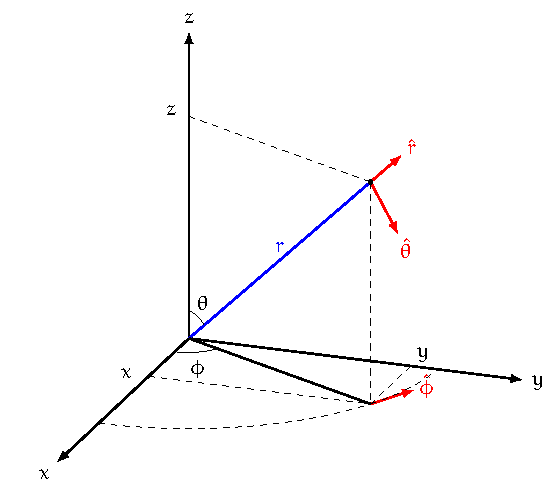
\includegraphics[width=10cm]{spherical_coordinates.pdf}

	\tdplotsetmaincoords{70}{110}
	%
	\pgfmathsetmacro{\thetavec}{48.17}
	\pgfmathsetmacro{\phivec}{63.5}
	%
	
	\begin{tikzpicture}[tdplot_main_coords]
		%Axis
		\draw[axis] (0,0,0) -- (6.5,0,0) node [pos=1.1] {$x$};
		\draw[axis] (0,0,0) -- (0,6,0) node [pos=1.05] {$y$};
		\draw[axis] (0,0,0) -- (0,0,5.5)  node [pos=1.05] {$z$};   
		
		%Unit Vectors
%		\tdplotsetcoord{p}{1}{90}{\phivec}
%    	\draw[univec] (2,4,0) -- ($(p)+(2,4,0)$) node [pos=1.35] {$\vu*{\varpi}$};
		\tdplotsetcoord{P'}{7}{\thetavec}{\phivec}
    	\draw[univec] (0,0,0) -- (P') node [pos=1.05] {$\hat{r}$};
    	\tdplotsetcoord{P''}{1}{90}{90+\phivec}
    	\draw[univec] (2,4,0) -- ($(P'') + (2,4,0)$) node [pos=1.3] {$\hat{\phi}$};
    	\tdplotsetcoord{P'''}{1}{90+\thetavec}{\phivec}
    	\draw[univec] (2,4,4) -- ($(P''') + (2,4,4)$) node [pos=1.3] {$\hat{\theta}$};
		
		%Vectors
		\tdplotsetcoord{P}{6}{\thetavec}{\phivec}
		\draw[vec] (0,0,0) -- (P) node [midway, above] {$r$};
		\draw[thick] (0,0,0) -- (2,4,0);
		
		%Help Lines
		\draw[dashed] (2,4,4) -- (2,4,0);
		\draw[dashed] (2,0,0) -- (2,4,0) node [pos=-0.1] {$x$};
		\draw[dashed] (0,4,0) -- (2,4,0) node [pos=-0.3] {$y$};
		\draw[dashed] (0,0,4) -- (2,4,4) node [pos=-0.1] {$z$};
		\draw[dashed, tdplot_main_coords] (4.47,0,0) arc (0:90:4.47);
		
		%Point
		\node[fill=black, circle, inner sep=0.8pt] at (2,4,4) {};
		
		%Angles
		\tdplotdrawarc{(0,0,0)}{0.7}{0}{\phivec}{below}{$\phi$}
		 
	    \tdplotsetthetaplanecoords{\phivec}
	    \tdplotdrawarc[tdplot_rotated_coords]{(0,0,0)}{0.5}{0}{\thetavec}{}{}
	    \node at (0,0.25,0.67) {$\theta$};
		
	\end{tikzpicture}
\end{center}
\begin{center}
  	\tdplotsetmaincoords{70}{110}
	%
	\pgfmathsetmacro{\thetavec}{48.17}
	\pgfmathsetmacro{\phivec}{63.5}
	%
	
	\begin{tikzpicture}[tdplot_main_coords]
		%Axis
		\draw[axis] (0,0,0) -- (6,0,0) node [pos=1.1] {$x$};
		\draw[axis] (0,0,0) -- (0,6,0) node [pos=1.05] {$y$};
		\draw[axis] (0,0,0) -- (0,0,5.5)  node [pos=1.05] {$z$};   
		
		%Help Lines
		\draw[dashed] (2,4,4) -- (2,4,0);
		\draw[dashed] (2,0,0) -- (2,4,0) node [pos=-0.1] {$x$};
		\draw[dashed] (0,4,0) -- (2,4,0) node [pos=-0.35, left] {$y$};
		\draw[dashed] (0,0,4) -- (2,4,4) node [pos=-0.1] {$z$};
		\draw[dashed, tdplot_main_coords] (4.47,0,0) arc (0:90:4.47);
		
		%Unit Vectors
		\tdplotsetcoord{P'}{1}{90}{\phivec}
    	\draw[univec] (2,4,0) -- ($(P')+(2,4,0)$) node [pos=1.3] {$\hat{\rho}$};
    	\tdplotsetcoord{P''}{1}{90}{90+\phivec}
    	\draw[univec] (2,4,0) -- ($(P'') + (2,4,0)$) node [pos=1.3] {$\hat{\phi}$};
    	
    	%Vectors
		\tdplotsetcoord{P}{6}{\thetavec}{\phivec}
		\draw[vec] (0,0,0) -- (P);
		\draw[thick] (0,0,0) -- (2,4,0) node [pos=0.6, above] {$\rho$};
		
		%Point
		\node[fill=black, circle, inner sep=0.8pt] at (2,4,4) {};
		
		%Angles
		\tdplotdrawarc{(0,0,0)}{0.7}{0}{\phivec}{below}{$\phi$}
		
	\end{tikzpicture}
\end{center}
\begin{center}
  \renewcommand{\arraystretch}{1.5}
  \begin{tabular}{c|c|c}
    Polar & Cylindrical & Spherical\\
    \hline\hline
    $\mathbf{s} = s(\rho,\phi)$ & $\mathbf{s} = s(\rho,\phi,z)$ & $\mathbf{s} = s(r,\phi,\theta)$\\
    $\mathbf{s} = \begin{pmatrix}\rho\cos\phi\\\rho\sin\phi\end{pmatrix}$ & $\mathbf{s} = \begin{pmatrix}\rho\cos\phi\\\rho\sin\phi\\z\end{pmatrix}$ & $\mathbf{s} = \begin{pmatrix}r\cos\phi\sin\theta\\r\sin\phi\sin\theta \\ r\cos\theta\end{pmatrix}$
  \end{tabular}
\end{center}
Here,\footnote{Physicists amirite?} $\phi$ denotes the polar angle and $\theta$ denotes the azimuthal angle. Notice that $\phi \in [0,2\pi)$ and $\theta \in [0,\pi]$.\newline

We can see that $\hat\rho$, $\hat\phi$, and $\hat\theta$ in spherical coordinates are also position-dependent.
\begin{align*}
  \hat r &= \frac{\pd{\mathbf{s}}{r}}{\norm{\pd{\mathbf{s}}{r}}}\\
         &= \sin\theta\cos\phi\hat{i} + \sin\theta\sin\phi\hat{j} + \cos\theta\hat{k}\\
  \hat{\phi} &= \frac{\pd{\mathbf{s}}{\phi}}{\norm{\pd{\mathbf{s}}{\phi}}}\\
             &= -\sin\phi\hat{i} + \cos\phi\hat{j}\\
  \hat{\theta} &= \frac{\pd{\mathbf{s}}{\theta}}{\norm{\pd{\mathbf{s}}{\theta}}}\\
               &= \cos\phi\cos\theta\hat{i} + \cos\theta\sin\phi\hat{j} - \sin\theta\hat{k}
\end{align*}
\subsubsection{Scale Factors and Jacobians}%
\begin{center}
  \renewcommand{\arraystretch}{1.5}
  \begin{tabular}{c|c|c|c}
    Coordinate System & Line Element & Area Element & Volume Element\\
    \hline\hline
    Polar & $d \mathbf{s} = \hat\rho d\rho + \rho \hat\phi d\phi$ & $d\mathbf{a} = r\:drd\phi$ & ---\\
    Cylindrical & $d \mathbf{s} = \hat\rho d\rho + \rho\hat\phi d\phi + \hat k dz$ & --- & $d\tau = r\:dr d\phi dz$\\
    Spherical & $d \mathbf{s} = \hat r dr + r\sin\theta \hat\phi d\phi + r\hat\theta d\theta$ &  $d \mathbf{a} = r^2\sin\theta d\phi d\theta$ & $d\tau = r^2\sin\theta\:dr d\phi d\theta$
  \end{tabular}
\end{center}
In cylindrical coordinates, we can use the chain rule to find the value of $d \mathbf{r}$:
\begin{align*}
  d \mathbf{r} &= \hat{\rho}d\rho + \rho\hat\phi d\phi + \hat k dz.
\end{align*}
The extra factor of $\rho$ in the expression of $\rho\hat\phi d\phi$ is the \textit{scale factor} on $\phi$.\newline

Similarly, in spherical coordinates, we have
\begin{align*}
  d \mathbf{r} &= \hat{r} dr +  r\sin\theta \hat{\phi}d\phi + r\hat{\theta}d\theta,
\end{align*}
with scale factors of $r\sin\theta$ on $\hat\phi d\phi$ and $r$ on $\hat\theta d\theta$.\newline

When we go from line elements (of the form $d\mathbf{r}$) to area elements (of the form $d \mathbf{a}$), we can see that the area element in polar coordinates is $d \mathbf{a} = \rho d\rho d\phi$ --- we need the extra factor of $\rho$ to account for the fact that the magnitude of the area element scales with the radius.\newline

Similarly, the volume element in cylindrical coordinates is $d\tau = r dr d\phi dz$ and the volume element in spherical coordinates is $r^2 \sin \theta dr d\phi d\theta$.\newline

Recall that the definition of an angle $\phi$ that subtends an arc length $s$ is $\phi \frac{s}{r}$, where $r$ is the radius of a circle. We can imagine a similar concept on a sphere --- a \textit{solid angle} measured in steradians is of the form $\Omega = \frac{A}{r^2}$, where $A$ denotes the surface area subtended by the angle $\Omega$. In particular, since $d\Omega = \frac{dA}{r^2}$, we find that $d\Omega = \sin\theta d\phi d\theta$.\newline

When we are dealing with products of scale factors, we need to use the Jacobian to determine the proper scale factor on any given element:
\begin{align*}
  d\mathbf{a} &= dx dy\\
              &= \left\vert J \right\vert \:du dv,
\end{align*}
where $|J|$ denotes the determinant of the Jacobian matrix. We write the Jacobian as follows:
\begin{align*}
  J &= \frac{\partial \left(x,y\right)}{\partial \left(u,v\right)}\\
    &= \begin{pmatrix}\pd{x}{u} & \pd{y}{u}\\ \pd{x}{v} & \pd{y}{v}\end{pmatrix}.
\end{align*}
We specifically desire the determinant:
\begin{align*}
  |J| &= \pd{x}{u}\pd{y}{v} - \pd{y}{u}\pd{x}{v}.
\end{align*}
\subsection{Complex Numbers}%
\begin{center}
  \renewcommand{\arraystretch}{1.75}
  \begin{tabular}{c|c}
    Quantity & Expression and/or Criterion\\
    \hline\hline
    Cartesian form & $z = a + bi$\\
    Polar form & $z = re^{i\phi}$\\
    $r$ & $\sqrt{a^2 + b^2}$\\
    $\phi$ & $\arg z = \arctan\left(\frac{b}{a}\right)$\\
    \hline
    Cartesian $z^{\ast}$ & $z^{\ast} = a-bi$\\
    Polar $z^{\ast}$ & $z = re^{-i\phi}$\\
    $|z|$ & $\sqrt{zz^{\ast}}$\\
    \hline
    $\re(z)$ & $\re(z) = \frac{z + z^{\ast}}{2}$\\
    $\im(z)$ & $\im(z) = \frac{z - z^{\ast}}{2i}$\\
    $\cos\phi$ & $\frac{e^{i\phi} + e^{-i\phi}}{2}$\\
    $\sin\phi$ & $\frac{e^{i\phi} - e^{-i\phi}}{2i}$\\
    \hline
    $e^{i\phi}$ & $\cos \phi + i\sin\phi$\\
    $e^{in\phi}$ & $\cos \left(n\phi\right) + i\sin \left(n\phi\right)$
  \end{tabular}
\end{center}
\subsubsection{Introduction}%

\begin{center}
  \begin{tikzpicture}[scale = 2]
  \def\xmax{2.0}
  \def\ymax{1.6}
  \def\R{1.9}
  \def\ang{35}
  \coordinate (O) at (0,0);
  \coordinate (R) at (\ang:\R);
  \coordinate (-R) at (-\ang:\R);
  \coordinate (X) at ({\R*cos(\ang)},0);
  \coordinate (Y) at (0,{\R*sin(\ang)});
  \coordinate (-Y) at (0,{-\R*sin(\ang)});
  \node[fill=mydarkblue,circle,inner sep=0.8] (R') at (R) {};
  \node[fill=mydarkred,circle,inner sep=0.8] (-R') at (-R) {};
  \node[mydarkblue,above right=-2] at (R') {$z=a+bi=re^{i\phi}$};
  \node[mydarkred,below right=-1] at (-R') {$z^{\ast}=a-bi=re^{-i\phi}$};
  \draw[dashed,mydarkblue]
    (Y) -- (R') --++ (0,{0.1-\R*sin(\ang)});
  \draw[dashed,mydarkred]
    (-Y) -- (-R') --++ (0,{\R*sin(\ang)-0.45});
  \draw[->,line width=0.9] (-0.65*\xmax,0) -- (\xmax+0.05,0) node[right] {Re};
  \draw[->,line width=0.9] (0,-\ymax) -- (0,\ymax+0.05) node[left] {Im};
  \draw[vector] (O) -- (R') node[pos=0.55,above left=-2] {$r$};
  \draw[vector,myred] (O) -- (-R') node[pos=0.55,below left=-2] {$r$};
  \draw pic[->,"$\phi$",mydarkblue,draw=mydarkblue,angle radius=23,angle eccentricity=1.24]
    {angle = X--O--R};
  \draw pic[<-,"$-\phi$"{right=-1},mydarkred,draw=mydarkred,angle radius=20,angle eccentricity=1]
    {angle = -R--O--X};
  %\tick{X}{90} node[scale=0.9,left=6,below right=-2] {$x = r\cos\theta$};
  \tick{X}{90} node[scale=1,below=-1] {$x$};
  \tick{Y}{ 0} node[mydarkblue,scale=1,left] {$y$}; %r\sin\theta = 
  \tick{-Y}{ 0} node[mydarkred,scale=1,left] {$-y$};
\end{tikzpicture}
\end{center}
A complex number is denoted
\begin{align*}
  z &= a + bi
\end{align*}
where $i^2 = -1$ and $a,b\in \R$. This is known as the cartesian representation. However, we can also imagine $z$ as the polar representation:
\begin{align*}
  z &= re^{i\phi},
\end{align*}
where $\phi = \arg z$ is known as the argument, and $r = |z|$ is the modulus. We can see the relation between the cartesian and polar representations through Euler's identity:\footnote{This can be proven relatively easily through substitution into the Taylor series, which is allowed because $e^z$ is entire.}
\begin{align*}
  r\left(\cos \phi + i\sin\phi\right) &= re^{i\phi}.
\end{align*}
We denote the conjugate of $z$ as $z^{\ast}$\footnote{Physicists amirite?}, found by $z^{\ast} = a - bi = re^{-i\phi}$.\newline

We find $\re(z)$ and $\im(z)$, the real and imaginary parts of $z$, by
\begin{align*}
  \re(z) &= \frac{z + z^{\ast}}{2}\\
  \im(z) &= \frac{z - z^{\ast}}{2i}.
\end{align*}
We say that a complex number of the form $e^{i\phi}$ is a \textit{pure phase}, as $\left\vert e^{i\phi} \right\vert = 1$.\newline

To find if some complex number $z$ is purely real or purely imaginary, we can use the following criterion:
\begin{align*}
  z\in \R \Leftrightarrow z = z^{\ast}\\
  z\in i\R \Leftrightarrow z = -z^{\ast}.
\end{align*}
\begin{example}[Real, Imaginary, or Complex?]
  Consider
  \begin{align*}
    z_1 &= i^{i}.
  \end{align*}
  To find if this is purely real or complex, we take
  \begin{align*}
    z_1^{\ast} &= \left(-i\right)^{-i}\\
               &= \left(\frac{1}{-i}\right)^{i}\\
               &= i^{i}.
  \end{align*}
  Thus, $z_1\in \R$. In order to determine the value of $i^i$, we substitute the polar form:
  \begin{align*}
    z_1 &= \left(e^{i\frac{\pi}{2}}\right)^{i}\\
        &= e^{-\frac{\pi}{2}}.
  \end{align*}
\end{example}
\subsubsection{Some Trigonometry with Complex Exponentials}%
Consider $z = \cos \phi + i\sin\phi$. We can see that
\begin{align*}
  \re(z) &= \cos\phi\\
         &= \frac{\left(\cos \phi + i\sin\phi\right) + \left(\cos\phi - i\sin\phi\right)}{2}\\
         &= \frac{e^{i\phi} + e^{-i\phi}}{2}\\
  \im(z) &= \sin\phi\\
         &= \frac{\left(\cos\phi + i\sin\phi\right) - \left(\cos\phi - i\sin\phi\right)}{2i}\\
         &= \frac{e^{i\phi} - e^{-i\phi}}{2i}.
\end{align*}
We can actually define $\sin\phi$ and $\cos\phi$ with the above derivation.\newline

\begin{theorem}[De Moivre]
\begin{align*}
  e^{inx} &= \cos\left(nx\right) + i\sin \left(nx\right)\\
          &= \left(e^{ix}\right)^{n}\\
          &= \left(\cos x + i\sin x\right)^n.
\end{align*}
\end{theorem}
\begin{example}[Finding $\cos \left(2x\right)$ and $\sin \left(2x\right)$]
  \begin{align*}
    \cos\left(2x\right) + i\sin \left(2x\right) &= \left(\cos x + i\sin x\right)^2\\
                                                &= \left(\cos^2 x - \sin^2 x\right) + i\left(2\sin x \cos x\right).
  \end{align*}
  Since the real parts and imaginary parts have to be equal, this means
  \begin{align*}
    \cos 2x &= \cos^2 x - \sin^2 x\\
    \sin^2 x &= 2\sin x \cos x.
  \end{align*}
\end{example}
In particular, we can see that $e^{in\phi} = \left(-1\right)^n$ and $e^{in\frac{\pi}{2}} = i^n$.\footnote{This will be especially useful when we get to Fourier series.}\newline

Additionally, we can see that for $z = re^{i\phi}$,
\begin{align*}
  z^{1/m} &= \left(re^{i\phi + 2\pi n}\right)^{1/m}\\
          &= r^{1/m}e^{i\frac{1}{m}\left(\phi + 2\pi n\right)},
\end{align*}
where $n\in \N$ and $m$ is fixed. For $r = 1$, we call these values the $m$ roots of unity.
\begin{example}[Waves and Oscillations]
  Recall that for a wave with spatial frequency $k$, angular frequency $\omega$, and amplitude $A$, the wave is represented by
  \begin{align*}
    f(x,t) &= A\cos\left(kx - \omega t\right).
  \end{align*}
  The speed of a wave $v$ is equal to $\frac{\omega}{k}$.\newline

  Simple harmonic motion is characterized by the solution to the differential equation $\ddot{\mathbf{x}} = -\omega^2 \mathbf{x}$, where $\mathbf{x}$ denotes position. In simple harmonic motion, there is no spatial motion, meaning our function is only of time:
  \begin{align*}
    f(t) &= A\cos \omega t\\
         &= \re\left(Ae^{i\omega t}\right).
  \end{align*}
  As a result of the representation of complex numbers in polar form, we can do math entirely in exponentials, then take the real part of our solution to find $f(t)$.\newline

  Unfortunately, in the real world, there is friction; as a result, our oscillation is damped by an exponential factor.
\end{example}
\begin{example}[Hyperbolic Sine and Hyperbolic Cosine]
  We wish to calculate $\cos ix$ and $\sin ix$.
  \begin{align*}
    \cos ix &= \frac{1}{2}\left(e^{i\left(ix\right)} + e^{-i\left(ix\right)}\right)\\
            &= \frac{e^{-x} + e^{x}}{2}
  \end{align*}
  We define $\cosh x = \cos \left(ix\right)$. Additionally,
  \begin{align*}
    - i\sin ix &= -i\frac{1}{2i}\left(e^{i\left(ix\right)} - e^{-i\left(ix\right)}\right)\\
            &= i\frac{e^{x} - e^{-x}}{2i}.\\
            &= \frac{e^{x} - e^{-x}}{2}.
  \end{align*}
  We define $\sinh x = -i\sin\left(ix\right)$.\newline

  Similar to how $\cos^2 x + \sin^2 x = 1$, we can find that $\cosh^2 x - \sinh^2 x = 1$.
\end{example}
\subsection{Index Algebra}%
We usually denote vectors by either $\vec{A}$, $\mathbf{A}$, or
\begin{align*}
  \begin{pmatrix}a_1\\a_2\\\vdots\\a_n\end{pmatrix},
\end{align*}
which is defined by a basis.\newline

If we imagine we are in $n$-dimensional space, we can let $A_i$ where $i = 1,2,\dots,n$ denote both
\begin{itemize}
  \item the $i$th component of $\vec A$;
  \item the entire vector $\vec{A}$ (since $i$ can be arbitrary).
\end{itemize}
\subsubsection{Contractions and Dummy Indices}%
Consider $C = AB$, where $A,B $ are $n\times m$ and $m\times p$ matrices respectively.
\begin{align*}
  C &= \begin{pmatrix}A_{11} & A_{12} & \cdots & A_{1m}\\
  \vdots & \vdots & \ddots & \vdots\\
A_{n1} & A_{n2} & \cdots & A_{nm}\end{pmatrix} \begin{pmatrix}B_{11} & B_{12} & \cdots & B_{1p}\\
  \vdots & \vdots & \ddots & \vdots\\
B_{m1} & B_{m2} & \cdots & B_{mp}\end{pmatrix}.
\end{align*}
%The index notation description of this multiplication is much more contracted than the traditional method learned in linear algebra:
%\begin{align*}
%  C_{ij} &= \sum_{k=1}^{n} A_{ik}B_{kj}.
%\end{align*}
%This might seem like a very convoluted system for small matrices.\newline
%
%However, looking at $AB$ compared to $BA$, we see that
%\begin{align*}
%  \left(AB\right)_{ij} &= \sum_{k} A_{ik}B_{kj}\\
%                       &= \sum_{k}B_{kj}A_{ik},\\
%  \left(BA\right)_{ij} &= \sum_{k}B_{ik}A_{kj}\\
%                       &= \sum_{k}A_{kj}B_{ik}.
%\end{align*}
\begin{definition}[Matrix Multiplication in Index Notation]
  For matrices $A$ and $B$, where $A$ is an $m\times n$ and $B$ is a $n\times p$ matrix, we write
  \begin{align*}
    C_{ij} &= \sum_{k=1}^{n}A_{ik}B_{kj}
  \end{align*}
\end{definition}
We say that $k$ is a dummy index, since $k$ takes values from $1$ to $n$. Note that the value we calculate is $C_{ij}$; in other words, in the sum $\sum_{k}A_{ik}B_{kj}$, the indices of the form $ij$ are the ``net indices'' from the multiplication.\newline

Note that if $C = BA$, then
\begin{align*}
  C_{ij} &= \sum_{k=1}^{n}B_{ik}A_{kj}\\
         &= \sum_{k=1}^{n}A_{kj}B_{ik}\\
         &\neq \sum_{k=1}^{n}A_{ik}B_{kj}.
\end{align*}
The corresponding fact is that $AB\neq BA$ necessarily.\newline

Note that the index that is summed over always appears exactly twice.
\begin{definition}[Symmetric Matrix]
  Let $C$ be a matrix. Then, we say $C$ is symmetric if
  \begin{align*}
    C_{ij} &= C_{ji}
  \end{align*}
\end{definition}
\begin{definition}[Antisymmetric Matrix]
  Let $C$ be a matrix. We say $C$ is antisymmetric if
  \begin{align*}
    C_{ij} &= -C_{ji}.
  \end{align*}
\end{definition}
We can always decompose a random matrix into the sum of a symmetric matrix and an antisymmetric matrix.
\subsubsection{Two Special Tensors}%
\begin{center}
  \renewcommand{\arraystretch}{1.75}
  \begin{tabular}{c|c|c}
    Name & Notation & Definition\\
    \hline\hline
    Kronecker Delta & $\delta_{ij}$ &$\delta_{ij} = \begin{cases}1 & i=j\\ 0 & i\neq j \end{cases}$\\
    Levi--Civita Symbol & $\epsilon_{ijk}$ & $\epsilon_{ijk} = \begin{cases}1 & \text{$(i,j,k) = (1,2,3)$ cyclically}\\-1 & \text{$(i,j,k) = (2,1,3)$ cyclically}\\0 & \text{else} \end{cases}$
  \end{tabular}
\end{center}
\begin{center}
  \renewcommand{\arraystretch}{1.25}
  \begin{tabular}{c|c}
    Order of $\left(i,j,k\right)$ & Value of $\epsilon_{ijk}$\\
    \hline\hline
    $1,2,3$ & $1$\\
    $3,1,2$ & $1$\\
    $2,3,1$ & $1$\\
    \hline
    $1,3,2$ & $-1$\\
    $2,1,3$ & $-1$\\
    $3,2,1$ & $-1$\\
    \hline
    else & $0$
  \end{tabular}
\end{center}
\begin{center}
  \renewcommand{\arraystretch}{1.5}
  \begin{tabular}{c|c}
    Value & Index Notation\\
    \hline\hline
    $\mathbf{A}\times \mathbf{B}$ & $\displaystyle\sum_{i,j,k}\epsilon_{ijk}A_iB_j\hat{e}_k$\\
    $\left(\mathbf{A}\times \mathbf{B}\right)_{\ell}$  & $\displaystyle\sum_{i,j}\epsilon_{ij\ell}A_iB_j$\\
    $\left(\hat{e}_i \times \hat{e}_j\right)\cdot \hat{e}_{k}$ & $\epsilon_{ijk}$\\
    \hline
    $B_i$ & $\displaystyle\sum_{\alpha}B_{\alpha}\delta_{\alpha i}$\\
    $\mathbf{A}\cdot \mathbf{B}$ & $\displaystyle\sum_{i,j}A_iB_j\delta_{ij}$\\
    \hline
    $\displaystyle\sum_{j,k}\epsilon_{mjk}\epsilon_{njk}$ & $2\delta_{mn}$\\
    $\displaystyle\sum_{\ell}\epsilon_{mn\ell}\epsilon_{ij\ell}$ & $\delta_{mi}\delta_{nj} - \delta_{mj}\delta_{ni}$
  \end{tabular}
\end{center}
\begin{definition}[Kronecker Delta]
  The Kronecker Delta, $\delta_{ij}$, is the tensor that denotes the identity matrix.
  \begin{align*}
    \delta_{ij} &= \begin{cases}
      1 & i=j\\
      0 & i\neq j
    \end{cases}
  \end{align*}
\end{definition}
\begin{example}[Extracting an Index]
  Consider $A$ as vector. Then,
  \begin{align*}
    \sum_{i}A_i \delta_{ij} &= A_j.
  \end{align*}
  In other words, the Kronecker Delta collapses the sum to the $j$th index.
\end{example}
\begin{example}[Orthonormal Basis from Kronecker Delta]
  Let $\set{\hat{e}_i}_{i=1}^{n}$ be a basis for some vector space $V$. If
  \begin{align*}
    \hat{e}_i\cdot \hat{e}_j &= \delta_{ij}
  \end{align*}
  for every $i,j$, then $\set{\hat{e}_i}_{i=1}^{n}$ is an orthonormal basis for $V$.
\end{example}
\begin{definition}[Levi--Civita Symbol]
  In two dimensions, as a matrix, we write
  \begin{align*}
    \epsilon_{ij} &= \begin{pmatrix}0 & 1 \\ -1 & 0\end{pmatrix},
  \end{align*}
  meaning
  \begin{align*}
    \epsilon_{ij} &= \begin{cases}
      1 & i=1,j=2\\
      -1 & i=2,j=1\\
      0 & \text{else}
    \end{cases}.
  \end{align*}
  The Levi--Civita Symbol is antisymmetric, just as the Kronecker Delta is symmetric.\newline

  In three dimensions, we define
  \begin{align*}
    \epsilon_{ijk}  &= \begin{cases}
      1 & \text{$\left(i,j,k\right) = \left(1,2,3\right)$ cyclically}\\
      -1 & \text{$\left(i,j,k\right) = \left(2,1,3\right)$ cyclically}\\
      0 & \text{else}
    \end{cases}.
  \end{align*}
  In other words, $\epsilon_{ijk} = -\epsilon_{jik}$.
\end{definition}
\begin{exercise}[Relations between $\delta_{ij}$ and $\epsilon_{ijk}$]
  \begin{align*}
    \sum_{j,k}\epsilon_{mjk}\epsilon_{njk} &= 2\delta_{mn}\\
    \sum_{\ell}\epsilon_{mn\ell}\epsilon_{ijl} &= \delta_{mi}\delta_{nj} - \delta_{mj}\delta_{ni}
  \end{align*}
\end{exercise}
\begin{definition}[Dot Product]
  Let $\set{\hat{e}_i}_{i=1}^{n}$ be an orthonormal basis for $V$. Let $\mathbf{A} = \sum_{i}A_i\hat{e}_i$ and $\mathbf{B} = \sum_{i}B_i\hat{e}_i$. Then,
  \begin{align*}
    \mathbf{A}\cdot \mathbf{B} &= \sum_{i,j}\left(A_i\hat{e}_i\right)\cdot\left(B_j\hat{e}_j\right)\\
                               &= \sum_{i,j}A_iB_j \left(\hat{e}_i \cdot \hat{e}_j\right)\\
                               &= \sum_{i,j}A_iB_j \delta_{ij}\\
                               &= \sum_{i}A_iB_i
  \end{align*}
\end{definition}
\begin{definition}[Cross Product]
  Let $\set{\hat{e}_i}_{i=1}^{3}$ be the standard basis over $\R^3$. Let $\mathbf{A} = \sum_{i}A_i\hat{e}_i$ and $\mathbf{B} = \sum_{i}B_i\hat{e}_i$. Then,
  \begin{align*}
    \mathbf{A}\times \mathbf{B} &= \sum_{i,j}\left(A_i\hat{e}_i\right)\times \left(B_j\hat{e}_j\right)\\
                                &= \sum_{i,j}A_iB_j \left(\hat{e}_i \times \hat{e}_j\right)\\
                                &= \sum_{i,j,k}A_iB_j\left(\epsilon_{ijk}\hat{e}_k\right).
  \end{align*}
  Instead of asking about $\mathbf{A}\times \mathbf{B}$, we ask about $\left(\mathbf{A}\times \mathbf{B}\right)_{\ell}$, yielding
  \begin{align*}
    \left(\mathbf{A}\times \mathbf{B}\right)_{\ell} &= \left(\mathbf{A}\times \mathbf{B}\right)\cdot \hat{e}_{\ell}\\
                                                    &= \left(\sum_{i,j,k}A_iB_j\left(\epsilon_{ijk}\hat{e}_k\right)\right)\cdot \hat{e}_{\ell}\\
                                                    &= \sum_{i,j}\epsilon_{ij\ell}A_iB_j.
  \end{align*}
\end{definition}
\begin{remark}
  This notation for $\mathbf{A}\times \mathbf{B}$ automatically shows us that
  \begin{align*}
    \left(\mathbf{B}\times \mathbf{A}\right)_{\ell} &= \sum_{i,j}\epsilon_{ij\ell}B_iA_j\\
                                                    &= -\sum_{i,j}\epsilon_{ji\ell}B_iA_j\\
                                                    &= -\sum_{i,j}\epsilon_{ji\ell}A_jB_i\\
                                                    &= -\sum_{i,j}\epsilon_{ij\ell}A_iB_j\tag*{$i,j$ are dummy indices}\\
                                                    &= -\left(\mathbf{A}\times \mathbf{B}\right)_{\ell}.
  \end{align*}
\end{remark}
\begin{example}[Central Force and Angular Momentum]
  A central force is defined by
  \begin{align*}
    \mathbf{F} &= f(r)\hat{r},
  \end{align*}
  where $\hat{r}$ is a radial vector.\newline

  Angular momentum is defined by
  \begin{align*}
    \mathbf{L} &= \mathbf{r}\times \mathbf{p},
  \end{align*}
  where $\mathbf{r}$ denotes position and $\mathbf{p}$ denotes momentum. Then,
  \begin{align*}
    \frac{d\mathbf{L}}{dt} &= \frac{d}{dt}\left(\mathbf{r}\times \mathbf{p}\right)\\
                           &= \left(\frac{d}{dt}\mathbf{r}\times \mathbf{p}\right) + \mathbf{r}\times \left(\frac{d\mathbf{p}}{dt}\right)\\
                           &= m\left(\frac{d}{dt}\mathbf{r}\times \frac{d}{dt}\mathbf{r}\right) + \mathbf{r}\times \left(f(r)\hat{r}\right)\\
                           &= f(r)\left(\mathbf{r}\times \hat{r}\right).
  \end{align*}
  This implies that $\frac{d\mathbf{L}}{dt} = 0$ under a central force.
\end{example}
\begin{example}[Determinant]
  Let $\mathbf{M} = M_{ij}$ be square. We denote $\mathbf{M}_i$ to be the vector denoting the $i$th-row. Then,
  \begin{align*}
    m &= \left\vert \mathbf{M} \right\vert\\
      &= \mathbf{M}_1\cdot \left(\mathbf{M}_2 \times \mathbf{M}_3\right)\\
      &= \mathbf{M}_3 \cdot \left(\mathbf{M}_1\times \mathbf{M}_2\right)\\
      &= \mathbf{M}_2 \cdot \left(\mathbf{M}_3\times \mathbf{M}_1\right).
  \end{align*}
\end{example}
\begin{example}[Trace]
  Let $\mathbf{M} = M_{ij}$ be a square matrix. We define $\tr\left(\mathbf{M}\right) = \sum_{i}M_{ii}$. Equivalently,
  \begin{align*}
    \tr\left(\mathbf{M}\right) &= \sum_{ij}M_{ij}\delta_{ij}\\
                                     &= \sum_{i}M_{ii}.
  \end{align*}
  Note that
  \begin{align*}
    \tr\left(I_{n}\right) &= \sum_{i}\delta_{ii}\\
                                     &= n.
  \end{align*}
  When we upgrade to $3$ matrices, we take
  \begin{align*}
    \tr\left(ABC\right) &= \sum_{i,j}\left(\sum_{k,\ell}A_{ik}B_{k\ell}C_{\ell j}\right)\delta_{ij}\\
                        &= \sum_{i,k,\ell}A_{ik}B_{k\ell}C_{\ell i}\\
                        &= \sum_{i,k,\ell}C_{\ell i}A_{ik}B_{k\ell}\\
                        &= \tr\left(CAB\right).
  \end{align*}
  In other words, the trace is invariant under cyclic permutations.
\end{example}
\begin{example}[Moment of Inertia Tensor]\hfill
%  \begin{center}
%    \begin{tikzpicture}
%  \def\R{3.3}   % circle radius
%  \def\r{1.4}   % mass radius (inner sep)
%  \def\L{1.2}   % angular momentum
%  \def\v{0.8}   % velocity
%  \def\l{0.35}  % angular momentum
%  \def\ang{18}  % mass angular position
%  \def\angp{40} % angle to feign perspective
%  \coordinate (O) at (\ang+90+\angp:0.4*\R);
%  \coordinate (R1) at (\ang-180:0.8*\R);
%  \coordinate (R2) at (0,0);
%  \coordinate (R3) at (\ang:0.65*\R);
%  \coordinate (R1E) at ($(O)!1.25!(R1)$); % R1 extended
%  \draw[Lvec] (O) --++ (0,\L) node[below right=0] {$\vb{L}$};
%  \draw[xcol!80!black] (\ang-180:\R) -- (\ang:\R);
%  \draw[dashed] (R1) -- (R1E);
%  \draw[pvec] (R1) --++ (\ang:\v) node[below=1] {$\vb{p}$};
%  \draw[pvec] (R2) --++ (\ang:\v) node[below=1] {$\vb{p}$};
%  \draw[pvec] (R3) --++ (\ang:\v) node[below=1] {$\vb{p}$};
%  \node[mass,circle,inner sep=2] (R1') at (R1) {};
%  \node[mass,circle,inner sep=2] (R2') at (R2) {};
%  \node[mass,circle,inner sep=2] (R3') at (R3) {};
%  \draw[rvec] (O) -- (R1') node[midway,above left=-2] {$\vb{r}$};
%  \draw[rvec] (O) -- (R2') node[midway,below left=-3] {$\vb{r}_\mathrm{t}$};
%  \draw[rvec] (O) -- (R3') node[midway,above=-1] {$\vb{r}$};
%  \draw (R2)++(\ang-180:\l) --++ (\ang+90+\angp:\l) --++ (\ang:\l);
%  %\draw pic["$\theta$",draw,angle radius=24,angle eccentricity=1.24] {angle=R2--R1--O};
%  \draw pic["$\theta$",draw,angle radius=7,angle eccentricity=1.5] {angle=R1E--R1--R2};
%\end{tikzpicture}
%  \end{center}
  Recall that
  \begin{align*}
    \mathbf{L} &= \mathbf{r}\times \mathbf{p},\\
               &= I\boldsymbol{\omega}.
  \end{align*}
  where $\mathbf{p} = m\dot{\mathbf{x}}$, and $I$ denotes the moment of inertia. Note that $I\sim mr^2$. On a more fundamental level, it is the case that the first equation, $\mathbf{L} = \mathbf{r}\times \mathbf{p}$, is the ``true'' definition of $\mathbf{L}$.

  Consider a small portion $m_{\alpha}$ about some axis at radius $\mathbf{r}_{\alpha}$ and momentum $\mathbf{p}_{\alpha}$. Then, we have
  \begin{align*}
    \mathbf{L}_{\alpha} &= \sum_{\alpha}\mathbf{r}_{\alpha}\times \mathbf{p}_{\alpha}\\
                        &= \sum_{\alpha}m_{\alpha}\left(\mathbf{r}_{\alpha}\times \left(\boldsymbol{\omega}\times \mathbf{r}_{\alpha}\right)\right).
  \end{align*}
  In the infinitesimal case (i.e., as $\alpha \rightarrow 0$), we get
  \begin{align*}
    \mathbf{L} &= \int_{}^{} \mathbf{r}\times \left(\boldsymbol{\omega}\times \mathbf{r}\right)\rho\:d\tau,
  \end{align*}
  where $\rho$ denotes volume density. Applying the identity $\mathbf{A}\times \left(\mathbf{B}\times \mathbf{C}\right) = \mathbf{B}\left(\mathbf{A}\cdot \mathbf{C}\right) - \mathbf{C}\left(\mathbf{A}\cdot \mathbf{B}\right)$, we find
  \begin{align*}
    \mathbf{L} &= \int\left(\boldsymbol{\omega}\left(\mathbf{r}\cdot \mathbf{r}\right) - \mathbf{r}\left(\mathbf{r}\cdot \boldsymbol{\omega}\right)\right)\rho\:d\tau.
  \end{align*}
  Switching to index notation, we have
  \begin{align*}
    L_i &= \int_{}^{} \left(\omega_ir^2 - r_i\sum_{j}r_j\omega_j\right)\rho\:d\tau\\
        &= \sum_{j}\int_{}^{} \omega_j\left(\delta_{ij}r^2 - r_ir_j\right)\rho\:d\tau\\
        &= \sum_{j}\omega_j\underbrace{\left(\int_{}^{} \left(\delta_{ij}r^2 - r_ir_j\right)\rho\:d\tau\right)}_{\text{moment of inertia tensor}}\\
        &= \sum_{j}I_{ij}\omega_j.
  \end{align*}
\end{example}
\subsection{Binomial Theorem}%
The binomial theorem allows us to calculate the expansion
\begin{align*}
  \left(x+y\right)^n &= \sum_{m=0}^{n}{n\choose m}x^{n-m}y^{m}.
\end{align*}
In the case of $\left(x + y\right)^2 = x^2y^{0} + 2x^{1}y^1 + x^{0}y^2 = x^2 + 2xy + y^2$. Recall that
\begin{align*}
  {n\choose m} &= \frac{n!}{m!\left(n-m\right)!}.
\end{align*}
Recall that $0! = 1$.
\subsection{Infinite Series}%
Let
\begin{align*}
  S &= \sum_{k=0}^{\infty}a_k
\end{align*}
be an infinite series. We are often curious as to the convergence of this sum (for a variety of reasons). Formally, we have to invoke partial sums
\begin{align*}
  S_N &= \sum_{k=0}^{N}a_k,
\end{align*}
and see if the sequence of partial sums is convergent. However, we will prefer to use series convergence tests.

%In particular, we are interested in monotonically decreasing $a_k$.
\begin{example}[Geometric Series]
  Let
  \begin{align*}
    S &= \sum_{k=0}^{\infty}r^k\\
      &= 1 + r + r^2 + \cdots
  \end{align*}
  Then, we have
  \begin{align*}
    S_N &= \sum_{k=0}^{N}r^k\\
    rS_N &= \sum_{k=0}^{N}r^k.
  \end{align*}
  Subtracting, we get
  \begin{align*}
    (1-r)S_N &= 1-r^{N+1}\\
    S_N &= \frac{1-r^{N+1}}{1-r}.
  \end{align*}
  In the limit, we expect that if $r\rightarrow \infty$, and $r < 1$, then $r^{N+1} \rightarrow 0$. In the infinite case, we have
  \begin{align*}
    S &= \sum_{k=0}^{\infty}r^k\\
      &= \frac{1}{1-r},
  \end{align*}
  if $r < 1$.
\end{example}
There are a few prerequisites for series convergence:
\begin{itemize}
  \item there exists some $K$ for which for all $k \geq K$, $a_{k+1} \leq a_{k}$;
  \item $\lim_{k\rightarrow\infty} < \infty$;
  \item we need the series to reduce ``quickly'' enough.
\end{itemize}
\begin{example}[Ratio Test]
  A series $S = \sum_{k}a_k$ converges if the ratio of consecutive terms is (eventually) less than $1$:
  \begin{align*}
    r &= \lim_{k\rightarrow\infty}\frac{a_{k+1}}{a_k} < 1.
  \end{align*}
\end{example}
\begin{example}[Applying the Ratio Test]
  Consider $S = \sum_{k}\frac{1}{k!}$. Then,
  \begin{align*}
    r &= \lim_{k\rightarrow\infty}\frac{\frac{1}{(k+1)!}}{\frac{1}{k!}}\\
      &= \lim_{k\rightarrow\infty}\frac{1}{k+1}\\
      &= 0 < 1
  \end{align*}
\end{example}
\begin{example}[Riemann Zeta Function]
  We write
  \begin{align*}
    \zeta(s) &= \sum_{k=1}^{\infty}\frac{1}{k^s}.
  \end{align*}
  In order to evaluate the convergence of the Riemann zeta function. We have
  \begin{align*}
    r &= \lim_{k\rightarrow\infty}\frac{\frac{1}{(k+1)^s}}{\frac{1}{k^s}}\\
      &= \lim_{k\rightarrow\infty}\left(\frac{k}{k+1}\right)^s\\
      &= 1.
  \end{align*}
  Unfortunately, this means the ratio test is inconclusive.\newline

  For examples of evaluations of the zeta function, we have
  \begin{align*}
    \zeta(1) &= 1 + \frac{1}{2} + \frac{1}{3} + \cdots\\
    \zeta(2) &= 1 + \frac{1}{4} + \frac{1}{9} + \cdots\\
             &= \frac{\pi^2}{6}.
  \end{align*}
\end{example}
\begin{example}[Absolute Convergence]
  In our original ratio test, we had assumed that $a_k$ are real and positive. However, if the $a_k\in \C$, we have to look at the convergence in modulus:
  \begin{align*}
    r &= \lim_{k\rightarrow\infty}\left\vert \frac{a_{k+1}}{a_k} \right\vert.
  \end{align*}
  If $\sum_{k}\left\vert a_k \right\vert$ converges, this is known as absolute convergence.
\end{example}
\begin{example}[Alternating Series Test]
  If the series
  \begin{align*}
    \sum_{k=0}^{\infty}\left(-1\right)^ka_{k}
  \end{align*}
  has the following conditions:
  \begin{itemize}
    \item $a_{k+1} < a_k$ for $k > K$;
    \item $\lim_{k\rightarrow\infty}a_k = 0$;
  \end{itemize}
  then $\sum_{k}\left(-1\right)^ka_k$ converges.\newline

  For instance, the alternating harmonic series converges
  \begin{align*}
    \sum_{k=1}^{\infty}\left(-1\right)^{k+1}\frac{1}{k} &= \ln 2.
  \end{align*}
\end{example}
\subsubsection{Power Series}%
Consider the function
\begin{align*}
  S(x) &= \sum_{k=0}^{\infty}a_kx^k.
\end{align*}
This is a series both in $a_k$ and in $x$. In order to determine convergence, we use the ratio test as follows:
\begin{align*}
  \lim_{k\rightarrow\infty}\left\vert \frac{a_{k+1}x^{k+1}}{a_kx^k} \right\vert &= \left\vert x \right\vert\lim_{k\rightarrow\infty}\left\vert \frac{a_{k+1}}{a_k} \right\vert\\
                                                                                &\equiv \left\vert x \right\vert r.
\end{align*}
In particular, for convergence , it must be the case that
\begin{align*}
  \left\vert x \right\vert r < 1.
\end{align*}
We define
\begin{align*}
  R &= \begin{cases}
    \frac{1}{r} & 0 < r < \infty\\
    0 & r = \infty\\
    \infty & r = 0
  \end{cases}.
\end{align*}
In particular, this means
\begin{align*}
  |x| &< R.
\end{align*}
\begin{definition}[Radius of Convergence]
  For a power series $\sum_{k}a_kx^k$, the series converges for $|x| < R$,\footnote{The definition is not the true radius of convergence; it is actually that $r = \limsup_{k\rightarrow\infty}\sqrt[k]{\left|a_k\right|}$. It just happens to be the case that the ratio test and root test return the same value when they're regular limits (rather than limits superior).} where
  \begin{align*}
    r &= \lim_{k\rightarrow\infty}\left\vert \frac{a_{k+1}}{a_k} \right\vert\\
    R &= \begin{cases}
      \frac{1}{r} & 0 < r < \infty\\
      0 & r = \infty\\
      \infty & r=0
    \end{cases}.
  \end{align*}
\end{definition}
  Note that convergence for $|x| < R$ does not provide information regarding convergence at the boundary.
\begin{example}[Geometric Series]
  We have
  \begin{align*}
    \frac{1}{1-x} &= \sum_{k=0}^{\infty}x^k
  \end{align*}
  has $R = 1$, meaning the power series converges for $|x| < 1$.
\end{example}
\begin{example}[Exponential Function]
  We have
  \begin{align*}
    e^{x} &= \sum_{k=0}^{\infty}\frac{x^k}{k!},
  \end{align*}
  with $R = \infty$.
\end{example}
\begin{example}[Natural Log]
  We have
  \begin{align*}
    \ln\left(1+x\right) &= x - \frac{1}{2}x^2 + \frac{1}{3}x^{3} - \cdots
  \end{align*}
  In particular, since $R = 1$, we know that the radius of convergence is $|x| < 1$. However, the series does converge on the boundary when $x = 2$, but not when $x =0$ (for obvious reasons).
\end{example}
\begin{example}[Why Radius of Convergence?]
  Consider two series
  \begin{align*}
    \frac{1}{1-x^2} &= \sum_{k=0}^{\infty}x^{2k}\\
    \frac{1}{1+x^2} &= \sum_{k=0}^{\infty}\left(-1\right)^{k}x^{2k}.
  \end{align*}
  We can see that the first series converges for $|x| < 1$. However, even though $\frac{1}{1+x^2}$ has a domain across the entire real numbers, it is still the case that the \textit{series} converges for $|x| < 1$.\newline

  The primary reason that the radius of convergence is defined as such is because, over the complex numbers, it is the case that $x^2 + 1 = 0$ at $x = \pm i$, meaning $\frac{1}{1+z^2}$ has singularities at those values of $z$.
\end{example}
The main reason power series are useful is that, when truncated, they are simply polynomials. In particular, with power series, we can reverse the order of sum and derivative.
\subsubsection{Taylor Series}%
\begin{center}
  \renewcommand{\arraystretch}{1.5}
  \begin{tabular}{c|c}
    Function & Taylor Series\\
    \hline\hline
    $f(x)$ & $ \sum_{k=0}^{\infty}\frac{\left(x-x_0\right)^n}{n!}\left(\frac{d^{n}f}{dx^n}\biggr\vert_{x=x_0}\right)$\\
    $e^x$ & $\sum_{n=0}^{\infty}\frac{x^n}{n!}$\\
    $\cos x$ & $\sum_{n=0}^{\infty}\frac{\left(-1\right)^nx^{2n}}{\left(2n\right)!}$\\
    $\sin x$ & $\sum_{n=0}^{\infty}\frac{\left(-1\right)^{n+1}x^{2n+1}}{\left(2n+1\right)!}$\\
    $\left(1 + x\right)^{\alpha}$ & $\sum_{n=0}^{\infty}\frac{\left(\alpha\right)_{n}}{n!}x^n$\footnotemark
  \end{tabular}
  \footnotetext{We define $\left(\alpha\right)_n = \prod_{k=0}^{n-1}\left(\alpha - k\right)$}
\end{center}
\begin{definition}
  The Taylor series of a function $f(x)$ about $x_0$ is defined by
  \begin{align*}
    f(x) &= \sum_{n=0}^{\infty}\frac{\left(x-x_0\right)^n}{n!}\left(\frac{d^nf}{dx^n}\biggr\vert_{x=x_0}\right).
  \end{align*}
\end{definition}
\begin{remark}
  The reason we write $\frac{d^nf}{dx^n}$ is because $\frac{d^n}{dx^n}$ is an operator in and of itself.
\end{remark}
\begin{example}[The Most Important Taylor Series]
  \begin{align*}
    e^x &= \sum_{n=0}^{\infty}\frac{x^n}{n!}\\
    \cos x &= \sum_{n=0}^{\infty}\frac{\left(-1\right)^nx^{2n}}{\left(2n\right)!}\\
    \sin x &= \sum_{n=0}^{\infty}\frac{\left(-1\right)^{n+1}x^{2n+1}}{\left(2n+1\right)!}
  \end{align*}
\end{example}
\begin{example}[Equilibrium Points]
  Let $U(x)$ denote a potential over $x$. Then, $\mathbf{F} = -\nabla U$. We have
  \begin{align*}
    U(x) &= U(x_0) + \left(x-x_0\right)U'\left(x_0\right) + \frac{1}{2!}\left(x-x_0\right)^2U''\left(x_0\right) + \frac{1}{3!}\left(x-x_0\right)^3U'''\left(x_0\right) + \cdots
  \end{align*}
  When we analyze an equilibrium point, we disregard the $U\left(x_0\right)$ term, and see that the derivative of $U$ is zero; thus, we can truncate our series at the second derivative close to $x=x_0$:
  \begin{align*}
    U(x) &\approx \frac{1}{2}U''\left(x_0\right)\left(x-x_0\right)^2\\
         &= \frac{1}{2}m\omega^2 \left(x-x_0\right)^2.
  \end{align*}
  In other words, when we are very close to equilibrium, we have simple harmonic motion.
\end{example}
\begin{example}[Faster Taylor Series]
  Consider the function
  \begin{align*}
    \exp \left(\frac{x}{1-x}\right).
  \end{align*}
  In order to create its Taylor series, we can create this Taylor series piecewise:
  \begin{align*}
    \exp\left(\frac{x}{1-x}\right) &= 1 + \left(\frac{x}{1-x}\right) + \frac{1}{2!}\left(\frac{x}{1-x}\right)^2 + \frac{1}{3!}\left(\frac{x}{1-x}\right)^3.
    \intertext{Now, we expand the denominators as geometric series:}
                                   &= 1 + x\left(\sum_{k=0}^{\infty}x^k\right) + \frac{x^2}{2!}\left(\sum_{k=0}^{\infty}x^k\right)^2 + \frac{x^3}{3!}\left(\sum_{k=0}^{\infty}x^k\right) + \cdots
                                   \intertext{If we want to expand through $x^3$, we have to expand by keeping track of \textit{every} term:}
                                   &= 1 + x + \frac{3}{2}x^2 + \frac{13}{6}x^3 + O\left(x^4\right).
  \end{align*}
  We say we have expanded the series through the third order; the lowest order correction, denoted $O\left(x^n\right)$, is the fourth order (in this case).
\end{example}
\begin{example}[Exponentiated Operator]
  Consider a (square) matrix $M$. Then, we define
  \begin{align*}
    e^{M} &= \sum_{k=0}^{\infty}\frac{M^k}{k!},
  \end{align*}
  where $M^k = \prod_{i=1}^{k}M$; we define $M^0 = I$. Similarly,
  \begin{align*}
    e^{\frac{d}{dx}} &= \sum_{k=0}^{\infty}\frac{d^k}{dx^k} \frac{1}{k!}.
  \end{align*}
  In particular, $e^{\frac{d}{dx}}$ is the Taylor series operator.
\end{example}
\begin{remark}
  In quantum mechanics, the momentum operator is
  \begin{align*}
    P &= -i\hbar \frac{d}{dx}.
  \end{align*}
\end{remark}
\begin{example}[Binomial Expansion]
  For any $\alpha \in \C$ and $|x| < 1$, we have
  \begin{align*}
    \left(1+x\right)^{\alpha} &= 1 + \alpha x + \frac{\alpha\left(\alpha - 1\right)}{2!}x^2 + \frac{\alpha\left(\alpha - 1\right)\left(\alpha - 2\right)}{3!}x^3 + \cdots
  \end{align*}
  Note that if $\alpha \in \Z^{+}$, then the series truncates (and we recover the binomial theorem again).\newline

  The main use of the binomial expansion is with very small quantities. For instance,
  \begin{align*}
    E &\sim \frac{1}{\left(x^2 + a^2\right)^{3/2}}\\
      &= \frac{1}{x^3\left(1 + \frac{a^2}{x^2}\right)^{3/2}}\\
      &\approx \frac{1}{x^3}\left(1-\frac{3}{2}\frac{a^2}{x^2}\right)\tag*{For $x \gg a$}
  \end{align*}
\end{example}
\begin{remark}
  The binomial expansion only applies to the form $\left(1 + x\right)^{\alpha}$. If we are dealing with an expression of the form $\left(a + x\right)^{\alpha}$, we need to factor out $a$, making the expression $a^{\alpha}\left(1 + x/a\right)^{\alpha}$.
\end{remark}
\begin{example}[Special Relativity with the Binomial Expansion]
  In the theory of special relativity, Einstein came up with the equations
  \begin{align*}
    E &= \gamma mc^2\\
    \gamma &= \frac{1}{\sqrt{1 - \frac{v^2}{c^2}}}.
  \end{align*}
  We can use the binomial expansion to find more information about $\gamma$.
  \begin{align*}
    E &= \left(1-\frac{v^2}{c^2}\right)^{-1/2}mc^2\\
      &= \left(1 + \frac{1}{2}\frac{v^2}{c^2} + \frac{\left(-\frac{1}{2}\right)\left(-\frac{3}{2}\right)}{2!}\left(-\frac{v^2}{c^2}\right)^{2} + \cdots\right)mc^2\\
      &= mc^2 + \underbrace{\frac{1}{2}mv^2\left(1 + \frac{3}{4}\frac{v^2}{c^2} + \frac{5}{8}\left(\frac{v^2}{c^2}\right)^{2} + \cdots\right)}_{\text{Kinetic Energy}}
  \end{align*}
  As we take $v \ll c$, we only need to keep the first order term in the expansion, meaning we have $E = mc^2 + \frac{1}{2}mv^2$.\newline

  Thus, we can find kinetic energy as $KE = \left(\gamma - 1\right)mc^2$. Notice that this means that \textit{most} energy is internal energy emergent as mass.
\end{example}
\subsection{Ten Integration Techniques}%
While Mathematica may exist,\footnote{Citation needed.} it is still valuable to know how to take various integrals. More importantly, knowing how to take integrals provides valuable insights into \textit{what} exactly integrals are.
\subsubsection{Integration by Parts}%
\begin{definition}[Integration by Parts]
  Using the product rule, we have
  \begin{align*}
    \int_{}^{} \frac{d}{dx}\left(uv\right)\:dx &= \int_{}^{} \frac{du}{dx}v - \frac{dv}{dx}u\:dx\\
                                               &= \int_{}^{} \frac{du}{dx}v\:dx - \int_{}^{} \frac{dv}{dx}u\:dx.
  \end{align*}
  Thus, we get
  \begin{align*}
    \int_{}^{} u\:dv &= uv - \int_{}^{} v\:du.
  \end{align*}
  In the case where our integrals are definite, we have
  \begin{align*}
    \int_{a}^{b} u\:dv &= uv\bigr\vert_{a}^{b} - \int_{a}^{b} v\:du.
  \end{align*}
  We say $uv\bigr\vert_{a}^{b}$ is the boundary term (or surface term).\footnote{We can also use integration by parts to define the (weak) derivative, assuming the boundary term is zero.}
\end{definition}
\begin{example}
  \begin{align*}
    \int_{}^{} xe^{ax}\:dx &= \frac{1}{a}xe^{ax} - \int_{}^{} \frac{1}{a}e^{ax}\:dx\tag*{$u = x$, $dv = e^{ax}dx$}\\
                           &= \frac{1}{a}xe^{ax} - \frac{1}{a^2}e^{ax}\\
                           &= \frac{1}{a^2}e^{ax}\left(ax - 1\right).
  \end{align*}
  The $+C$ is implicit.
\end{example}
\begin{example}
  \begin{align*}
    \int_{}^{} \ln x\:dx &= x\ln x - \int_{}^{} x\left(\frac{1}{x}\right)\:dx\tag*{$u = \ln x$, $dv = dx$}\\
                         &= x\ln x - x.
  \end{align*}
\end{example}
\subsubsection{Change of Variables}%
\begin{definition}[$u$-Substitution]
  Let $x = x(u)$, meaning $dx = \frac{dx}{du}du$. Thus, we get
  \begin{align*}
    \int_{x_1}^{x_2} f(x)\:du &= \int_{u(x_1)}^{u(x_2)} f\left(x(u)\right)\frac{dx}{du}\:du.
  \end{align*}
\end{definition}
\begin{example}
  \begin{align*}
    I_1 &= \int_{0}^{\infty} xe^{-ax^2}\:dx\\
        &= \frac{1}{2}\int_{0}^{\infty} e^{-au}\:du\tag*{$u = x^2$}\\
        &= \frac{1}{2a}
  \end{align*}
\end{example}
\begin{example}
  \begin{align*}
    \int_{0}^{\pi} \sin\theta\:d\theta &= \int_{-1}^{1} \:du\tag*{$u = \cos\theta$}\\
                                       &= 2.
  \end{align*}
  More generally, we have, for $f(\theta) = f(\cos\theta)$,
  \begin{align*}
    \int_{0}^{\pi} f(\theta)\sin\theta\:d\theta &= \int_{-1}^{1} f(u)\:du.
  \end{align*}
\end{example}
\begin{example}[Trig Substitution]
  \begin{align*}
  \int_{0}^{a} \frac{x}{x^2 + a^2}\:dx &= \int_{0}^{\pi/4} \frac{a^2\tan\theta\sec^2\theta}{a^2\left(1 + \tan^2\theta\right)}\:d\theta\tag*{$x = a\tan\theta$}\\
                                       &= \int_{0}^{\pi/4} \tan\theta\:d\theta\\
                                       &= -\ln\left(\cos\theta\right)\bigr\vert_{0}^{\pi/4}\\
                                       &= \ln\left(\sqrt{2}\right)\\
                                       &= \frac{1}{2}\ln(2).
  \end{align*}
\end{example}
\begin{example}[Trig Substitution 2.0]
  For rational functions of $\sin\theta$ and $\cos\theta$, we can use the half-angle trig substitution $u = \tan(\theta/2)$.\footnote{$\tan(\theta/2) = \frac{\sin\theta}{1 + \cos\theta}$} This yields
  \begin{align*}
    d\theta &= \frac{2du}{1 + u^2}\\
    \sin\theta &= \frac{2u}{1 + u^2}\\
    \cos\theta &= \frac{1-u^2}{1 + u^2}.
  \end{align*}
  For instance,
  \begin{align*}
    \int_{}^{} \frac{1}{1+\cos\theta}\:d\theta &= \int_{}^{} \frac{1}{1 + \frac{1-u^2}{1+u^2}}\frac{2}{1 + u^2} \:du\\
                                               &= \int_{}^{} \:du\\
                                               &= \tan(\theta/2)\\
                                               &= \frac{\sin\theta}{1 + \cos\theta}.
  \end{align*}
\end{example}
  %%%%%%%%%%%%%%%%%%%%%%%%%%%%%%%%%%%%%%%%%%%%%%%%%%%%%%%%%%%%%%%%
%
% Welcome to Overleaf --- just edit your LaTeX on the left,
% and we'll compile it for you on the right. If you open the
% 'Share' menu, you can invite other users to edit at the same
% time. See www.overleaf.com/learn for more info. Enjoy!
%
%%%%%%%%%%%%%%%%%%%%%%%%%%%%%%%%%%%%%%%%%%%%%%%%%%%%%%%%%%%%%%%
% Author: Izaak Neutelings (March 2019)
\documentclass[border=3pt,tikz]{standalone}
\tikzset{>=latex} % for LaTeX arrow head
\usepackage{pgfplots} % for the axis environment
\pgfplotsset{
  compat=1.13, % TikZ coordinates <-> axes coordinates
  /pgf/number format/1000 sep={},
  legend image code/.code={
    \draw[mark repeat=2,mark phase=2]
    plot coordinates {(0cm,0cm) (0.22cm,0cm) (0.44cm,0cm)};%
  }
} 
\usepackage{siunitx}

% redraw axis on top
\makeatletter \newcommand{\pgfplotsdrawaxis}{\pgfplots@draw@axis} \makeatother
\pgfplotsset{axis line on top/.style={after end axis/.append code={\pgfplotsdrawaxis}}
}

% CUSTOM COLORS
% See https://tikz.net/blackbody_color/
\definecolor{1000K}{rgb}{1,0.0337,0}
\definecolor{2000K}{rgb}{1,0.2647,0.0033}
\definecolor{3000K}{rgb}{1,0.4870,0.1411}
\definecolor{4000K}{rgb}{1,0.6636,0.3583}
\definecolor{5000K}{rgb}{1,0.7992,0.6045}
\definecolor{6000K}{rgb}{1,0.9019,0.8473}
\definecolor{8000K}{rgb}{0.7874,0.8187,1}
\definecolor{10000K}{rgb}{0.6268,0.7039,1}
\pgfdeclareverticalshading{rainbow}{100bp}{
  color(0bp)=(red); color(25bp)=(red); color(35bp)=(yellow);
  color(45bp)=(green); color(55bp)=(cyan); color(65bp)=(blue);
  color(75bp)=(violet); color(100bp)=(violet)
}
\colorlet{myred}{red!70!black}
\colorlet{mygreen}{green!70!black}
\colorlet{mydarkgreen}{green!55!black}

% PLANCK & RAYLEIGH-JEANS
% 2hc^2/lambda^5 = 2 * 6.62607015e-34 * 299792458^2
%                = 1.191042972e-16
%    W.m -> kW.nm: 1.191042972e26
%  hc/k lambda T = 6.62607015e-34*299792458/(1.38064852e-23)
%                = 0.01438777378
%         m -> nm: 0.01438777378e9
% 2ckT/lambda^4  = 2 * 299792458 * 1.38064852e-23
%                = 8.278160269e-15
%    W.m -> kW.nm: 8.278160269e18
\pgfmathdeclarefunction{planck}{2}{%
  \pgfmathparse{1.191042972e26/(#1^5)/(exp(0.01439e9/(#1*#2))-1)}%
}
\pgfmathdeclarefunction{rayleighjeans}{2}{%
  \pgfmathparse{8.278160269e18*#2/(#1^4)}%
}
\pgfmathdeclarefunction{wien}{2}{%
  \pgfmathparse{1.191042972e26/(#1^5)*exp(-0.01439e9/(#1*#2))}%
}
\pgfmathdeclarefunction{lampeak}{1}{% % Wien's displacement law
  \pgfmathparse{2.898e6/#1}%
}

\usepackage{newpxtext,eulerpx}
\begin{document}


% BLACK BODY - 3000, 4000, 5000K
\begin{tikzpicture}
  \message{^^JBlack body}
  \def\N{60}
  \def\xmax{3100}
  \def\ymax{1.36e10}
  \def\tick#1#2{\draw[thick] (#1+.01*\ymax) -- (#1-.01*\ymax) node[below=-.5pt,scale=0.75] {#2};}
  \begin{axis}[
      every axis plot/.style={
        mark=none,samples=\N,domain=5:\xmax,smooth},
      xmin=(-.05*\xmax), xmax=(1.05*\xmax),
      ymin=(-.08*\ymax), ymax=(1.08*\ymax),
      restrict y to domain=0:\ymax,
      axis lines=middle,
      axis line style=thick,
      %enlargelimits=upper, % extend the axes a bit to the right and top
      tick style={black,thick},
      ticklabel style={scale=0.8},
      %xtick style={draw=none},xticklabels=none,
      max space between ticks=26,
      xlabel={Wavelength $\lambda$ [nm]},
      ylabel={Power $P$ [kW/sr\,m$^2$\,nm]},
      xlabel style={at={(rel axis cs:0.5,0)},below=-1pt,font=\small},
      ylabel style={at={(rel axis cs:-0.11,0.5)},rotate=90},
      width=9cm, height=7cm,
      %clip=false
      tick scale binop=\times,
      every y tick scale label/.style={at={(rel axis cs:0,1)},anchor=south}]
    ]
    
    % RAINBOW
    \shade[shading=rainbow,shading angle=90,opacity=0.5] (380,0) rectangle (740,\ymax);
    \node[above=-1pt,scale=0.8] at (200,\ymax) {\strut UV}; % 10 - 400 nm
    \node[above=-1pt,scale=0.8] at (570,\ymax) {\strut optical}; % 380 - 740 nm
    \node[above=-1pt,scale=0.8] at (920,\ymax) {\strut IR}; % 740 - 1050 nm
    
    % PLANCK
    \addplot[very thick,red]    {planck(x,3000)};
    \addplot[very thick,orange] {planck(x,4000)};
    \addplot[very thick,samples=3*\N,blue] {planck(x,5000)};
    %\addplot[dashed,thick,red,domain=1000:4000]    {rayleighjeans(x,3000)};
    %\addplot[dashed,thick,orange,domain=1000:4000] {rayleighjeans(x,4000)};
    \addplot[dashed,thick,blue,domain=1000:4000]   {rayleighjeans(x,5000)};
    %\addplot[dashed,thick,red,domain=1000:4000]    {wien(x,3000)};
    %\addplot[dashed,thick,orange,domain=1000:4000] {wien(x,4000)};
    %\addplot[dashed,thick,blue,domain=1000:4000]   {wien(x,5000)};
    
    %% MAXIMUM (Wien's displacement law)
    %\addplot[mygreen,very thin,variable=T,domain=2500:6000]
    %  ({lampeak(T)},{planck(lampeak(T),T)});
    
    % LABELS
    \node[above=0pt,scale=0.75,red] at (1150,{planck(1150,3000)}) {\SI{3000}{K}};
    \node[above right=-1pt,scale=0.75,orange!80!black] at (740,{planck(740,4000)}) {\SI{4000}{K}};
    \node[above right=-1pt,scale=0.75,blue] at (800,{planck(800,5000)}) {\SI{5000}{K}};
k    \node[above right=-1pt,scale=0.75,blue] at (1500,{rayleighjeans(1500,5000)}) {\SI{5000}{K} Rayleigh-Jeans};
    
    %% TICKS
    %\tick{500,0}{500}
    %\tick{1000,0}{1000}
    %\tick{1500,0}{1500}
    %\tick{2000,0}{2000}
    %\tick{2500,0}{2500}
    %\tick{3000,0}{3000}
    
  \end{axis}
\end{tikzpicture}


%% BLACK BODY - 3000, 4000, 5000K, Wien's displacement law
%\begin{tikzpicture}
%  \message{^^JBlack body, Wien's displacement law}
%  \def\N{60}
%  \def\xmax{3100}
%  \def\ymax{1.36e10}
%  \def\tick#1#2{\draw[thick] (#1+.01*\ymax) -- (#1-.01*\ymax) node[below=-.5pt,scale=0.75] {#2};}
%  \begin{axis}[
%      every axis plot/.style={
%        very thick,mark=none,samples=\N,domain=5:\xmax,smooth},
%      xmin=(-.05*\xmax), xmax=(1.05*\xmax),
%      ymin=(-.08*\ymax), ymax=(1.08*\ymax),
%      restrict y to domain=0:\ymax,
%      axis lines=middle,
%      axis line style=thick,
%      %enlargelimits=upper, % extend the axes a bit to the right and top
%      tick style={black,thick},
%      ticklabel style={scale=0.8},
%      %xtick style={draw=none},xticklabels=none,
%      max space between ticks=26,
%      xlabel={Wavelength $\lambda$ [nm]},
%      ylabel={Power $P$ [kW/sr\,m$^2$\,nm]},
%      xlabel style={at={(rel axis cs:0.5,0)},below=-1pt,font=\small},
%      ylabel style={at={(rel axis cs:-0.11,0.5)},rotate=90},
%      width=9cm, height=7cm,
%      %clip=false
%      tick scale binop=\times,
%      every y tick scale label/.style={at={(rel axis cs:0,1)},anchor=south}]
%    ]
%    
%    % RAINBOW
%    \shade[shading=rainbow,shading angle=90,opacity=0.5] (380,0) rectangle (740,\ymax);
%    \node[above=-1pt,scale=0.8] at (200,\ymax) {\strut UV}; % 10 - 400 nm
%    \node[above=-1pt,scale=0.8] at (570,\ymax) {\strut optical}; % 380 - 740 nm
%    \node[above=-1pt,scale=0.8] at (920,\ymax) {\strut IR}; % 740 - 1050 nm
%    
%    % PLANCK
%    \addplot[red]    {planck(x,3000)};
%    \addplot[orange] {planck(x,4000)};
%    \addplot[blue,samples=3*\N] {planck(x,5000)};
%    \addplot[dashed,thick,blue,domain=1000:3500] {rayleighjeans(x,5000)};
%    
%    % MAXIMUM (Wien's displacement law)
%    \addplot[mydarkgreen,thick,variable=T,domain=2200:4000,samples=40]
%      ({lampeak(T)},{planck(lampeak(T),T)});
%    \addplot[mydarkgreen,thick,variable=T,domain=4000:5200,samples=100]
%      ({lampeak(T)},{planck(lampeak(T),T)});
%    \fill[mydarkgreen!80!black] ({lampeak(3000)},{planck(lampeak(3000),3000)}) circle(1.5pt);
%    \fill[mydarkgreen!80!black] ({lampeak(4000)},{planck(lampeak(4000),4000)}) circle(1.5pt);
%    \fill[mydarkgreen!80!black] ({lampeak(5000)},{planck(lampeak(5000),5000)}) circle(1.5pt);
%    
%    % LABELS
%    \node[above=0pt,scale=0.75,red] at (1150,{planck(1150,3000)}) {\SI{3000}{K}};
%    \node[above right=-1pt,scale=0.75,orange!80!black] at (740,{planck(740,4000)}) {\SI{4000}{K}};
%    \node[above right=-1pt,scale=0.75,blue] at (800,{planck(800,5000)}) {\SI{5000}{K}};
%    \node[above right=-1pt,scale=0.75,blue] at (1500,{rayleighjeans(1500,5000)}) {\SI{5000}{K} Rayleigh-Jeans};
%    
%  \end{axis}
%\end{tikzpicture}
%
%
%% BLACK BODY - 3000, 4000, 5000K
%\begin{tikzpicture}
%  \message{^^JBlack body}
%  \def\N{60}
%  \def\xmax{3100}
%  \def\ymax{1.43e10}
%  \def\tick#1#2{\draw[thick] (#1+.01*\ymax) -- (#1-.01*\ymax) node[below=-.5pt,scale=0.75] {#2};}
%  \begin{axis}[
%      every axis plot/.style={
%        mark=none,samples=\N,domain=5:\xmax,smooth},
%      xmin=(0), xmax=(\xmax),
%      ymin=(0), ymax=(\ymax),
%      restrict y to domain=0:\ymax,
%      %axis lines=middle,
%      axis line style=thick,
%      tick style={black,thick},
%      ticklabel style={scale=0.8},
%      xlabel={Wavelength $\lambda$ [nm]},
%      ylabel={Power $P$ [kW/sr\,m$^2$\,nm]},
%      xlabel style={below=-1pt,font=\small},
%      ylabel style={above=-1pt},
%      width=9cm, height=7cm,
%      tick scale binop=\times,
%      every y tick scale label/.style={at={(rel axis cs:0,1)},anchor=south}]
%    ]
%    
%    % RAINBOW
%    \draw[dashed] (380,{planck(380,5000)}) -- (380,\ymax);
%    \draw[dashed] (740,{planck(740,5000)}) -- (740,\ymax);
%    \begin{scope}
%      \clip[variable=\x,domain=200:1000,samples=40]
%        plot(\x,{planck(\x,5000)}) |- (200,0) -- cycle;
%      \shade[shading=rainbow,shading angle=90,opacity=0.7] (380,0) rectangle (740,\ymax);
%    \end{scope}
%    
%    % PLANCK
%    \addplot[very thick,red]    {planck(x,3000)};
%    \addplot[very thick,orange] {planck(x,4000)};
%    \addplot[very thick,samples=3*\N,blue] {planck(x,5000)};
%    \addplot[dashed,thick,blue,domain=1000:4000]   {rayleighjeans(x,5000)};
%    
%    % MAXIMUM (Wien's displacement law)
%    \addplot[mydarkgreen,thick,variable=T,domain=2200:4000,samples=40]
%      ({lampeak(T)},{planck(lampeak(T),T)});
%    \addplot[mydarkgreen,thick,variable=T,domain=4000:5000,samples=100]
%      ({lampeak(T)},{planck(lampeak(T),T)});
%    \fill[mydarkgreen!80!black] ({lampeak(3000)},{planck(lampeak(3000),3000)}) circle(1.5pt);
%    \fill[mydarkgreen!80!black] ({lampeak(4000)},{planck(lampeak(4000),4000)}) circle(1.5pt);
%    \fill[mydarkgreen!80!black] ({lampeak(5000)},{planck(lampeak(5000),5000)}) circle(1.5pt);
%    
%    % LABELS
%    \node[above=0pt,scale=0.75,red]
%      at (1150,{planck(1150,3000)}) {\SI{3000}{K}};
%    \node[above right=-1pt,scale=0.75,orange!80!black]
%      at (740,{planck(740,4000)}) {\SI{4000}{K}};
%    \node[above right=-1pt,scale=0.75,blue]
%      at (800,{planck(800,5000)}) {\SI{5000}{K}};
%    \node[above right=-1pt,scale=0.75,blue]
%      at (1500,{rayleighjeans(1500,5000)}) {\SI{5000}{K} Rayleigh-Jeans};
%    
%    % LABELS
%    \node[below=2pt,scale=0.8] at (200,\ymax) {\strut UV}; % 10 - 400 nm
%    \node[below=2pt,scale=0.8] at (562,\ymax) {\strut optical}; % 380 - 740 nm
%    \node[below=2pt,scale=0.8] at (920,\ymax) {\strut IR}; % 740 - 1050 nm
%    
%  \end{axis}
%\end{tikzpicture}
%
%
%% BLACK BODY LOG-LOG - colors
%% See https://tikz.net/blackbody_color/
%\begin{tikzpicture} %[scale=2]
%  \message{^^JBlack body colors}
%  \def\N{40}
%  \def\xmin{35}
%  \def\xmax{1.7e5}
%  \def\ymin{1e2}
%  \def\ymax{2e12}
%  \begin{loglogaxis}[
%      every axis plot post/.append style={
%        very thick,mark=none,domain=\xmin:\xmax,samples=\N,smooth},
%      xmin=\xmin, xmax=(1.01*\xmax),
%      ymin=\ymin, ymax=\ymax,
%      restrict y to domain=0.1*\ymin:\ymax,
%      log basis y=10,
%      axis line style=thick,
%      tick style={black,thick},
%      ticklabel style={scale=0.8},
%      max space between ticks=23,
%      yminorticks=false,
%      xlabel={Wavelength $\lambda$ [nm]},
%      ylabel={Power $P$ [kW/sr\,m$^2$\,nm]},
%      xlabel style={at={(rel axis cs:0.5,0)},below=8pt},
%      ylabel style={above=-2pt},
%      legend style={at={(0.98,0.95)},anchor=north east,draw=none,fill=none,
%                    nodes={scale=0.7, transform shape}},
%      legend cell align={left},
%      width=8cm, height=6cm,
%      axis line on top
%    ]
%    
%    % RAINBOW
%    \shade[shading=rainbow,shading angle=90,opacity=0.5] (380,\ymin) rectangle (740,\ymax);
%    
%    % PLANCK
%    \addplot[10000K] {planck(x,10000)};
%    \addplot[6000K]  {planck(x,7500)};
%    \addplot[5000K]  {planck(x,5000)};
%    \addplot[3000K]  {planck(x,3000)};
%    \addplot[2000K]  {planck(x,2000)};
%    \addplot[1000K]  {planck(x,1000)};
%    \addplot[black]  {planck(x, 500)};
%    %\addplot[dashed,thick,black] {rayleighjeans(x,500)};
%    
%    % LEGENDS
%    \addlegendentry{\SI{10000}{K}}
%    \addlegendentry{\SI{7500}{K}}
%    \addlegendentry{\SI{5000}{K}}
%    \addlegendentry{\SI{3000}{K}}
%    \addlegendentry{\SI{2000}{K}}
%    \addlegendentry{\SI{1000}{K}}
%    \addlegendentry{\SI{500}{K}}
%    
%  \end{loglogaxis}
%\end{tikzpicture}
%
%
%% BLACK BODY LOG-LOG - Rayleigh-Jeans / Wien, 300K
%\begin{tikzpicture}
%  \message{^^JRayleigh-Jeans / Wien, 300K}
%  \def\N{40}
%  \def\xmin{1.5e3}
%  \def\xmax{2e6}
%  \def\ymin{5e-4}
%  \def\ymax{3e4}
%  \begin{loglogaxis}[
%      every axis plot/.style={
%        very thick,mark=none,domain=\xmin:\xmax,samples=\N,smooth},
%      xmin=\xmin, xmax=(1.01*\xmax),
%      ymin=\ymin, ymax=\ymax,
%      restrict y to domain=0.1*\ymin:\ymax,
%      log basis y=10,
%      axis line style=thick,
%      tick style={black,thick},
%      ticklabel style={scale=0.8},
%      %ticks=none,
%      max space between ticks=23,
%      yminorticks=false,
%      xlabel={Wavelength $\lambda$ [nm]},
%      ylabel={Power $P$ [kW/sr\,m$^2$\,nm]},
%      xlabel style={at={(rel axis cs:0.5,0)},below=8pt},
%      ylabel style={above=-2pt},
%      width=8cm, height=6cm,
%      legend style={at={(0.14,0.15)},anchor=south west,draw=none,fill=none,font=\small},
%      legend cell align={left},
%      axis line on top
%    ]
%  	
%    % PLANCK
%    \addplot[black]      {planck(x,300)};
%    \addplot[thick,blue] {rayleighjeans(x,300)};
%    \addplot[thick,red]  {wien(x,300)};
%    
%    % LEGENDS
%    \addlegendentry{Planck}
%    \addlegendentry{Rayleigh-Jeans}
%    \addlegendentry{Wien}
%    \node[scale=1] at (0.18*\xmax,0.01*\ymax) {$T=\SI{300}{K}$};
%    
%  \end{loglogaxis}
%\end{tikzpicture}
%
%
%% BLACK BODY LOG-LOG - Rayleigh-Jeans / Wien, 3000K
%\begin{tikzpicture}
%  \message{^^JRayleigh-Jeans / Wien, 3000K}
%  \def\N{40}
%  \def\xmin{1.5e2}
%  \def\xmax{2e5}
%  \def\ymin{5e1}
%  \def\ymax{4e9}
%  \begin{loglogaxis}[
%      every axis plot/.style={
%        very thick,mark=none,domain=\xmin:\xmax,samples=\N,smooth},
%      xmin=\xmin, xmax=(1.01*\xmax),
%      ymin=\ymin, ymax=\ymax,
%      restrict y to domain=0.1*\ymin:\ymax,
%      log basis y=10,
%      axis line style=thick,
%      tick style={black,thick},
%      ticklabel style={scale=0.8},
%      %ticks=none,
%      max space between ticks=23,
%      yminorticks=false,
%      xlabel={Wavelength $\lambda$ [nm]},
%      ylabel={Power $P$ [kW/sr\,m$^2$\,nm]},
%      xlabel style={at={(rel axis cs:0.5,0)},below=8pt},
%      ylabel style={above=-2pt},
%      width=8cm, height=6cm,
%      legend style={at={(0.14,0.15)},anchor=south west,draw=none,fill=none,font=\small},
%      legend cell align={left},
%      axis line on top
%    ]
%    
%    % RAINBOW
%    \shade[shading=rainbow,shading angle=90,opacity=0.1] (380,\ymin) rectangle (740,\ymax);
%  	
%    % PLANCK
%    \addplot[black]      {planck(x,3000)};
%    \addplot[thick,blue] {rayleighjeans(x,3000)};
%    \addplot[thick,red]  {wien(x,3000)};
%    
%    % LEGENDS
%    \addlegendentry{Planck}
%    \addlegendentry{Rayleigh-Jeans}
%    \addlegendentry{Wien}
%    \node[scale=1] at (0.17*\xmax,0.01*\ymax) {$T=\SI{3000}{K}$};
%    
%  \end{loglogaxis}
%\end{tikzpicture}
%
%
%% BLACK BODY LOG-LOG - Rayleigh-Jeans / Wien
%\begin{tikzpicture}
%  \message{^^JRayleigh-Jeans / Wien}
%  \def\N{40}
%  \def\xmin{3e2}
%  \def\xmax{2e6}
%  \def\ymin{1e-3}
%  \def\ymax{1e7}
%  \begin{loglogaxis}[
%      every axis plot/.style={
%        very thick,mark=none,domain=\xmin:\xmax,samples=\N,smooth},
%      xmin=\xmin, xmax=(1.01*\xmax),
%      ymin=\ymin, ymax=\ymax,
%      restrict y to domain=0.1*\ymin:\ymax,
%      log basis y=10,
%      axis line style=thick,
%      tick style={black,thick},
%      ticklabel style={scale=0.8},
%      %ticks=none,
%      max space between ticks=23,
%      yminorticks=false,
%      xlabel={Wavelength $\lambda$ [nm]},
%      ylabel={Power $P$ [kW/sr\,m$^2$\,nm]},
%      xlabel style={at={(rel axis cs:0.5,0)},below=9pt},
%      ylabel style={above=-2pt},
%      width=8cm, height=6cm,
%      axis line on top,
%      legend style={at={(0.65,0.9)},anchor=north west,draw=none,fill=none,font=\small}%,
%      %legend cell align={left},
%    ]
%    
%    % RAINBOW
%    \shade[shading=rainbow,shading angle=90,opacity=0.5] (380,\ymin) rectangle (740,\ymax);
%  	
%    % PLANCK
%    \addplot[blue]  {planck(x,800)};
%    \addplot[red]   {planck(x,300)};
%    \addplot[black] {planck(x,100)};
%    \addplot[dashed,thick,black] {rayleighjeans(x,100)};
%    \addplot[dashed,thick,red]   {rayleighjeans(x,300)};
%    \addplot[dashed,thick,blue]  {rayleighjeans(x,800)};
%    \addplot[dotted,thick,black] {wien(x,100)};
%    \addplot[dotted,thick,red]   {wien(x,300)};
%    \addplot[dotted,thick,blue]  {wien(x,800)};
%    
%    % LEGENDS
%    \addlegendentry{\SI{800}{K}}
%    \addlegendentry{\SI{300}{K}}
%    \addlegendentry{\SI{100}{K}}
%    
%  \end{loglogaxis}
%\end{tikzpicture}
%
%
%% BLACK BODY LOG-LOG - CMB redshift
%\begin{tikzpicture}
%  \message{^^JCMB redshift}
%  \def\N{60}
%  \def\xmin{5e1}
%  \def\xmax{2e8}
%  \def\ymin{1e-10}
%  \def\ymax{1e11}
%  \begin{loglogaxis}[
%      every axis plot/.style={
%        very thick,mark=none,samples=\N,smooth},
%      xmin=\xmin, xmax=(1.01*\xmax),
%      ymin=\ymin, ymax=\ymax,
%      restrict y to domain=0.1*\ymin:\ymax,
%      log basis y=10,
%      axis line style=thick,
%      tick style={black,thick},
%      ticklabel style={scale=0.8},
%      %ticks=none,
%      max space between ticks=23,
%      yminorticks=false,
%      variable=x,
%      xlabel={Wavelength $\lambda$ [nm]},
%      ylabel={Power $P$ [kW/sr\,m$^2$\,nm]},
%      xlabel style={at={(rel axis cs:0.5,0)},below=9pt},
%      ylabel style={above=-2pt},
%      width=8cm, height=6cm,
%      axis line on top
%    ]
%    
%    % BANDS
%    % See https://tikz.net/electromagnetic_spectrum/
%    \fill[violet!80!black!5] (\xmin,\ymin) rectangle (380,\ymax); % ultraviolet
%    \shade[shading=rainbow,shading angle=90,opacity=0.5] (380,\ymin) rectangle (740,\ymax);
%    \fill[red!80!black!4] (740,\ymin) rectangle (1e6,\ymax); % infrared
%    \fill[orange!80!black!4] (1e6,\ymin) rectangle (1e8,\ymax); % microwave
%    \fill[green!80!black!4] (1e8,\ymin) rectangle (\xmax,\ymax); % radio
%    \node[below=3,scale=0.7,violet!50!black] at ({\xmin*10^(log10(380/\xmin)/2)},\ymax) {UV};
%    \node[below=3,scale=0.7,red!50!black] at ({740*10^(log10(1e6/740)/2)},\ymax) {infrared};
%    \node[below=3,scale=0.7,orange!60!black] at ({1e6*10},\ymax) {microwave};
%  	
%    % PLANCK
%    \addplot[domain=\xmin:1e5,red]     {planck(x,3000)};
%    \addplot[domain=1e5:\xmax,red]     {rayleighjeans(x,3000)}; % prevent rounding errors in tail
%    \addplot[domain=2e5:\xmax,mygreen] {planck(x,2.725)};
%    
%    % LABELS
%    \node[above right=-1,red] at (1e4,{planck(1e4,3000)}) {\SI{3000}{K}};
%    \node[anchor=-70,mygreen] at (1e6,{planck(1e6,2.725)}) {\SI{2.725}{K}};
%    
%    % ARROW
%    \draw[->,line width=2,myred] (7e3,1e2) --++ (-42:17mm)
%      node[pos=0.38,above,sloped,scale=0.95] {redshift}
%      node[pos=0.38,below,sloped,scale=0.90] {$z\sim1100$};
%    
%  \end{loglogaxis}
%\end{tikzpicture}
%
%
%% BLACK BODY LOG-LOG - CMB temperature variations
%% https://en.wikipedia.org/wiki/Cosmic_microwave_background#Relationship_to_the_Big_Bang
%% T ~ 2.725 K with anisotropic variations of ~ 18 uK = 0.000018 K
%\begin{tikzpicture}
%  \message{^^JCMB temperature variations}
%  \def\N{40}
%  \def\xmin{3.2e5}
%  \def\xmax{8e6}
%  \def\ymin{5e-9}
%  \def\ymax{1e-6}
%  \begin{loglogaxis}[
%      every axis plot post/.append style={
%        very thick,mark=none,samples=\N,domain=\xmin:\xmax,smooth},
%      xmin=\xmin, xmax=(1.01*\xmax),
%      ymin=\ymin, ymax=\ymax,
%      restrict y to domain=0.1*\ymin:\ymax,
%      log basis y=10,
%      axis line style=thick,
%      tick style={black,thick},
%      ticklabel style={scale=0.8},
%      xtick={5e5,1e6,2e6,5e6},
%      minor xtick={4e5,6e5,7e5,8e5,9e5,3e6,4e6,6e6},
%      log number format code/.code={
%        \pgfkeys{/pgf/fpu}
%        \pgfmathparse{exp(\tick)}
%        \pgfmathprintnumber[sci,sci zerofill,precision=0]{\pgfmathresult}
%        \pgfkeys{/pgf/fpu=false}
%      },
%      xlabel={Wavelength $\lambda$ [nm]},
%      ylabel={Power $P$ [kW/sr\,m$^2$\,nm]},
%      xlabel style={at={(rel axis cs:0.5,0)},below=9pt},
%      ylabel style={above=-2pt},
%      width=8cm, height=6cm,
%      axis line on top,
%      legend style={
%        at={(0.24,0.3)},anchor=south west,draw=none,fill=none,font=\small},
%      legend cell align={left},
%      legend image code/.code={
%        \draw[mark repeat=2,mark phase=2]
%        plot coordinates {(0cm,0cm) (0.28cm,0cm) (0.56cm,0cm)};%
%      }
%    ]
%  	
%    % PLANCK
%    \addplot[red,dashed]  {planck(x,2.750)};
%    \addplot[mygreen]     {planck(x,2.725)};
%    \addplot[blue,dashed] {planck(x,2.700)};
%    \addplot[red,dashed]  {planck(x,2.750)}; % draw over 2.725
%    
%    % LEGENDS
%    \addlegendentry{\SI{2.750}{K}}
%    \addlegendentry{\SI{2.725}{K}}
%    \addlegendentry{\SI{2.700}{K}}
%    
%  \end{loglogaxis}
%\end{tikzpicture}


\end{document}

\begin{example}[Dimensionless Integrals]\hfill
  \begin{center}
    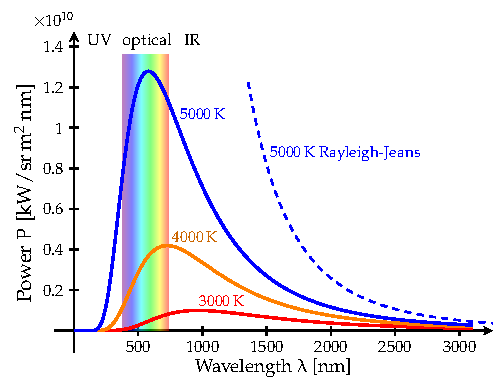
\includegraphics[width=10cm]{images/blackbody.pdf}
  \end{center}
  Anything that has a nonzero absolute temperature radiates some energy. In particular, we want to know how this radiation is distributed among various wavelengths.\newline

  For a box of photons in equilibrium at temperature $T$, the energy per volume per wavelength $\lambda$\footnote{read as (energy per volume) per wavelength} is
  \begin{align*}
    u\left(\lambda\right) &= \frac{8\pi h c}{\lambda^{5}\left(e^{h c/\lambda kT} - 1\right)}.
  \end{align*}
  Here, $h$ denotes Planck's constant, $c$ is the speed of light, and $k$ is Boltzmann's constant.\newline

  In order to find the total energy density, we have to integrate $u(\lambda)$ over all possible values of $\lambda$:
  \begin{align*}
    U &= \int_{0}^{\infty} u\left(\lambda\right)\:d\lambda\\
      &= 8\pi h c\int_{0}^{\infty}\frac{1}{\lambda^{5}\left(e^{hc/\lambda k T} - 1\right)} \:d\lambda
  \end{align*}
  This integral is, for lack of a better word, hard. However, if we remove the dimensions of $\lambda$ by substituting $x = \frac{hc}{\lambda k t}$, we can verify that the value of $U$ now becomes
  \begin{align*}
    U &= 8\pi h c \left(\frac{kT}{hc}\right)^{4}\underbrace{\int_{0}^{\infty} \frac{x^3}{e^x-1}\:dx}_{\text{scalar}}.
  \end{align*}
  Thus, all the physics\footnote{Who cares about that stuff?} is captured as a coefficient on the integral; namely, this integral captures the Stefan--Boltzmann law, which has that energy density scales by $T^{4}$.\newline

  Using some fancy techniques we will learn later, we can evaluate
  \begin{align*}
    \int_{0}^{\infty} \frac{x^3}{e^x-1}\:dx &= \frac{\pi^4}{15}.
  \end{align*}
\end{example}
\subsubsection{Even/Odd}%
\begin{definition}[Even and Odd Functions]
A function $f(x)$ is
\begin{itemize}
  \item even if $f(-x) = f(x)$;
  \item odd if $f(-x) = -f(x)$.
\end{itemize}
\end{definition}
Just as a matrix can be decomposed into a sum of a symmetric and antisymmetric matrix, we can decompose a function into a sum of an even function and an odd function.\newline

Integrals over symmetric intervals on functions with definite parity are very simple:
\begin{align*}
  \int_{-a}^{a} f(x)\:dx &= \begin{cases}
    2\int_{0}^{a} f(x)\:dx & f\text{ odd}\\
    0 & f\text{ even}
  \end{cases}.
\end{align*}
For the case of a function $g\left(x\right) = g\left(|x|\right)$, we have
\begin{align*}
  \int_{-a}^{b} g\left(|x|\right)\:dx &= \int_{-a}^{0} g(-x)\:dx + \int_{0}^{b} g(x)\:dx.
\end{align*}
\subsubsection{Products and Powers of Sines and Cosines}%
\begin{center}
  \renewcommand{\arraystretch}{1.5}
  \begin{tabular}{c|c}
    Value & Expression\\
    \hline
    $\sin\left(\alpha \pm \beta\right)$ & $\sin\alpha\cos\beta \pm \sin\beta\cos\alpha$\\
    $\cos\left(\alpha \pm \beta\right)$ & $\cos\alpha\cos\beta \mp \sin\alpha\sin\beta$\\
    \hline
    $\sin\alpha\cos\beta$ & $\frac{1}{2}\left(\sin(\alpha + \beta) + \sin\left(\alpha - \beta\right)\right)$\\
    $\cos\alpha\cos\beta$ & $\frac{1}{2}\left(\cos(\alpha - \beta) + \cos(\alpha + \beta)\right)$\\
    $\sin\alpha\sin\beta$ & $\frac{1}{2}\left(\cos(\alpha - \beta) - \cos(\alpha + \beta)\right)$
  \end{tabular}
\end{center}
\begin{example}
  If we have an integral
  \begin{align*}
    \int_{}^{} \sin(3x)\cos(2x)\:dx &= \frac{1}{2}\int_{}^{} \sin(5x) + \sin(x)\:dx\\
                                    &= \frac{1}{2}\left(-\frac{1}{5}\cos (5x) - \cos(x) \right).
  \end{align*}
\end{example}
\begin{center}
  \renewcommand{\arraystretch}{1.5}
  \begin{tabular}{c|c}
    Integral & Shortcut\\
    \hline
    $\int \sin^{m}(x)\cos^{2k+1}(x)\:dx$ & $\int_{}^{} u^{m}\left(1-u^2\right)^{k}\:du$\\
    $\int_{}^{} \sin^{2k+1}(x)\cos^{n}(x)\:dx$ & $-\int_{}^{} \left(1-u^2\right)^ku^{n}\:du$\\
    $\int_{}^{} \sin^{2}(x)\:dx$ & $\frac{x}{2} - \frac{1}{4}\sin(2x)$\\
    $\int_{}^{} \cos^{2}\left(x\right)\:dx$ & $\frac{x}{2} + \frac{1}{4}\sin(2x)$
  \end{tabular}
\end{center}
\begin{example}
  To evaluate
  \begin{align*}
    \int_{}^{} \sin^{2}(x)\:dx,\\
    \int_{}^{} \cos^2(x)\:dx
  \end{align*}
  we use the identity
  \begin{align*}
    \sin^2(x) &= \frac{1}{2}\left(1-\cos(2x)\right)\\
    \cos^{2}(x) &= \frac{1}{2}\left(1 + \cos(2x)\right),
  \end{align*}
  and take
  \begin{align*}
    \int_{}^{} \sin^2(x)\:dx &= \frac{1}{2}\int_{}^{} \left(1-\cos(2x)\right)\:dx\\
                             &= \frac{x}{2} - \frac{1}{4}\sin(2x)\\
    \int_{}^{} \cos^2(x)\:dx &= \frac{1}{2}\int_{}^{} \left(1+\cos(2x)\right)\:dx\\
                             &= \frac{x}{2} + \frac{1}{4}\sin(2x).
  \end{align*}
  Thus, we can see that
  \begin{align*}
    \int_{0}^{\pi} \sin^2(x)\:dx&= \frac{\pi}{2}\\
    \int_{0}^{\pi} \cos^2(x)\:dx&= \frac{\pi}{2}
  \end{align*}
\end{example}
\subsubsection{Axial and Spherical Symmetry}%
Consider a function of the form $f(x,y) = x^2 + y^2$. If we were to integrate with respect to $dx dy$, we would need a two dimensional integral. With polar coordinates, though, we would have $dx dy = rdrd\phi$. Since $f$ is axially symmetric, we would have our $dx dy = 2\pi r dr$, which is a one-dimensional integral.\newline

If we have something with spherical symmetry, then there is no dependence on either $\theta$ or $\phi$, yielding a function $f\left(\mathbf{r}\right) = f(r)$, meaning
\begin{align*}
  \int_{}^{} f\left(\mathbf{r}\right)\:d\tau &= \int_{}^{} f(r)r^2\sin\theta\:drd\theta d\phi\\
                                             &= 4\pi \int_{}^{} f(r)r^2\:dr.
\end{align*}
Note that $\int_{}^{} \sin\theta \:d\theta d\phi$ over the sphere is $4\pi$.
\begin{example}
  Consider a surface $S$ with charge density $\sigma\left(\mathbf{r}\right)$. Finding the total charge requires evaluating
  \begin{align*}
    Q &= \int_{S}^{} \sigma\left(\mathbf{r}\right)\:dA.
  \end{align*}
  If $S$ is hemispherical with $z > 0$ with radius $R$, and $\sigma = k\frac{x^2 + y^2}{R^2}$, the integrand is axially symmetric.\newline

  Using spherical coordinates, we evaluate
  \begin{align*}
    Q &= \int_{S}^{} \sigma\left(\mathbf{r}\right)\:dA\\
      &= \frac{k}{R^2}\int_{}^{} x^2 + y^2\:dA\\
      &= \frac{k}{R^2}\int_{}^{} \left(R^2\sin^2\theta\cos^2\phi + R^2\sin^2\theta\sin^2\phi\right)R^2\sin\theta\:d\theta d\phi\\
      &= kR^2\int_{S}^{} \sin^{3}\theta\:d\theta d\phi\\
      &= 2\pi kR^2 \int_{0}^{\pi/2} \sin^{3}\theta\:d\theta\\
      &= \frac{4\pi kR^2}{3}.
  \end{align*}
\end{example}
\begin{example}
  Let
  \begin{align*}
    \Phi\left(\mathbf{r}\right) &= \int_{}^{} \frac{e^{-i\mathbf{k}\cdot\mathbf{r}}}{\left(2\pi\right)^3\norm{\mathbf{k}}^2}\:d^{3}k
  \end{align*}
  where $k$-space is an abstract $3$-dimensional Euclidean space. In Cartesian coordinates, $d^3k = dk_x dk_y dk_z$, which yields the integral
  \begin{align*}
    \Phi\left(\mathbf{r}\right) &= \int_{}^{} \frac{e^{-ik_x x}e^{-ik_y y}e^{-ik_z z}}{\left(2\pi\right)^3 \left(k_x^2 + k_y^2 + k_z^2\right)}\:dk_x dk_y dk_z.
  \end{align*}
  This integral is very hard to evaluate (over Cartesian coordinates, anyway),\footnote{Citation needed.} so we need to use some other methods.\newline

  In spherical coordinates, we have $d^3 k = k^2 dk d\Omega$, yielding
  \begin{align*}
    \Phi\left(\mathbf{r}\right) &= \frac{1}{\left(2\pi\right)^3}\int_{}^{} k^2\frac{e^{-ikr\cos\theta}}{k^2}\:dkd\left(\cos \theta\right)d\phi.
  \end{align*}
  Since we are summing away all our $k$-dependence, we can orient $r$ along the $k_z$ axis. Thus, we can evaluate the integral as
  \begin{align*}
    \Phi\left(\mathbf{r}\right) &= \frac{1}{\left(2\pi\right)^3}\int_{}^{} k^2\frac{e^{-ikr\cos\theta}}{k^2}\:dkd\left(\cos \theta\right)d\phi\\
                                &= \frac{1}{\left(2\pi\right)^{2}}\int_{-1}^{1}\int_{0}^{\infty} e^{-ikr\cos\theta} \:dk d(\cos\theta)\\
                                &= \frac{1}{\left(2\pi\right)^2}\int_{}^{} \frac{1}{\left(-ikr\right)}\left(e^{-ikr} - e^{ikr}\right)\:dk\\
                                &= \frac{1}{\left(2\pi\right)^2}\int_{0}^{\infty}\frac{2\sin(kr)}{kr} \:dk\\
                                &= \frac{1}{2\pi^2}\underbrace{\int_{0}^{\infty} \frac{\sin(kr)}{kr}\:dk}_{\text{sinc integral}}.
  \end{align*}
  In order to evaluate the sinc integral, we have to use some different techniques.
\end{example}
\subsubsection{Differentiation with Respect to a Parameter}%
\begin{example}
  We can evaluate
  \begin{align*}
    \int_{}^{} xe^{ax}\:dx &= \pd{}{a}\left(\int_{}^{} e^{ax}\:dx\right)\\
                           &= \pd{}{a} \left(\frac{1}{a}e^{ax}\right)\\
                           &= -\frac{1}{a^2}e^{ax} + \frac{1}{a}xe^{ax}\\
                           &= \frac{1}{a^2}e^{ax}\left(ax - 1\right)
  \end{align*}
  When differentiating with respect to a parameter, it is important to remember that we are often differentiating \textit{with respect to the parameter}, not with respect to our main variable.
\end{example}
\begin{example}[Introducing a Parameter]
  We wish to solve the sinc integral,
  \begin{align*}
    \int_{0}^{\infty} \frac{\sin x}{x}\:dx.
  \end{align*}
  In order to do this, we will introduce a parameter such that differentiation will cancel out the $x$ in the denominator:
  \begin{align*}
    J\left(\alpha\right) &= \int_{0}^{\infty} e^{-\alpha x}\frac{\sin x}{x}\:dx. \tag*{$\alpha > 0$}
  \end{align*}
  In particular, $\alpha > 0$. We calculate
  \begin{align*}
    \frac{dJ}{d\alpha} &= -\int_{0}^{\infty} e^{-\alpha x}\sin x\:dx\\
                       &= -\frac{1}{1 + \alpha^2}.
  \end{align*}
  Therefore,
  \begin{align*}
    J\left(\alpha\right) &= -\int_{}^{} \frac{1}{\alpha^2}\:d\alpha\\
                         &= -\arctan\left(\alpha\right) + C.
  \end{align*}
  In order to determine the value of $C$, we need to make sure $J(\infty) = 0$. Therefore, $C = \frac{\pi}{2}$. Therefore, we have
  \begin{align*}
    J(0) &= \frac{\pi}{2}.
  \end{align*}
\end{example}
\subsubsection{Gaussian Integral}%
We cannot evaluate $I_0 = \int_{0}^{\infty} e^{-ax^2}\:dx$ using elementary methods, because $e^{-ax^2}$ is not an elementary function. The reason we care a lot about $e^{-ax^2}$ is because it is very important in quantum mechanics and statistics.\footnote{Who cares about that?}\newline

It is clear that $I_0$ converges. We can see that the dimension of $a$ is $x^{-2}$, and since we are integrating with respect to $dx$, we can see that our integral is related to $\frac{1}{\sqrt{a}}$.
\begin{example}
  We will not solve for $I_0$, but for $I_0^2$. Thus, we have
  \begin{align*}
    I_0^2 &= \left(\frac{1}{2}\int_{-\infty}^{\infty} e^{-ax^2}\:dx\right)\left(\frac{1}{2}\int_{-\infty}^{\infty} e^{-ay^2}\:dy\right)\\
          &= \frac{1}{4}\int_{-\infty}^{\infty}\int_{-\infty}^{\infty} e^{-a\left(x^2 + y^2\right)}\:dxdy\\
          &= \frac{1}{4}\int_{0}^{2\pi}\int_{0}^{\infty} re^{-ar^2}\:drd\phi\\
          &= \frac{\pi}{2}\int_{0}^{\infty} re^{-ar^2}\:dr\\
          &= \frac{\pi}{2}\left(\frac{1}{2}\int_{0}^{\infty} e^{-au}\:du\right)\\
          &= \frac{\pi}{4a}.
  \end{align*}
  Therefore, $I_0 = \frac{1}{2}\sqrt{\frac{\pi}{a}}$.
\end{example}
\begin{definition}[Family of Gaussian Integrals]
\begin{align*}
  I_n &= \int_{0}^{\infty} x^ne^{-ax^2}\:dx.
\end{align*}
\end{definition}
\begin{center}
  \renewcommand{\arraystretch}{1.5}
  \begin{tabular}{c|c}
    Expression & Value\\
    \hline
    $I_0$ & $\frac{1}{2}\sqrt{\frac{\pi}{a}}$\\
    $I_1$ & $\frac{1}{2a}$\\
    $I_{2n}$ & $(-1)^{n}\frac{d^{n}}{da^{n}}I_0$\\
    $I_{2n+1}$ & $\left(-1\right)^{n}\frac{d^{n}}{da^{n}}I_1$
  \end{tabular}
\end{center}
It is important to note that there are different expressions for the Gaussian integral:
\begin{align*}
  \int_{}^{} e^{-ax^2}\:dx\\
  \int_{}^{} e^{-a^2x^2}\:dx\\
  \int_{}^{} e^{-a^2x^2/2}\:dx\\
  \int_{}^{} e^{-x^2/a}\:dx\\
  \int_{}^{} e^{-x^2/a^2}\:dx,
\end{align*}
meaning we have to be careful when evaluating these integrals.
\begin{example}[Error Function]
Consider the integral
\begin{align*}
  \int_{0}^{53} e^{-ax^2}\:dx.
\end{align*}
Unfortunately, there is no way to do this integral analytically. It is only able to be calculated numerically.\newline

We define
\begin{align*}
  \text{erf}\left(u\right) &= \int_{0}^{u} e^{-ax^2}\:dx
\end{align*}
\end{example}
\subsubsection{Completing the Square}%
\begin{example}
  Consider the integral
  \begin{align*}
    \int_{-\infty}^{\infty} e^{-ax^2-bx}\:dx.
  \end{align*}
  This integral is Gaussian-esque, but it isn't fully Gaussian, yet.\newline

  To do this, we will complete the square:
  \begin{align*}
    ax^2 + bx &= a\left(x^2 + \frac{b}{a}x\right)\\
              &= a\left(x^2 + \frac{b}{a}x + \frac{b^2}{4a^2} - \frac{b^2}{4a^2}\right)\\
              &= a\left(x + \frac{b}{2a}\right)^2 - \frac{b^2}{4a}.
  \end{align*}
  In particular, this turns the integral into
  \begin{align*}
    \int_{-\infty}^{\infty} e^{-ax^2 - bx}\:dx &= \int_{-\infty}^{\infty} e^{-a\left(x + b/2a\right)^2 + b^2/4a}\:dx\\
                                               &= e^{b^2/4a}\int_{-\infty}^{\infty} e^{-a\left(x + b/2a\right)}\:dx\\
                                               &= e^{b^2/4a}\left(\sqrt{\frac{\pi}{a}}\right)\\
                                               &= e^{b^2/4a}\sqrt{\frac{\pi}{a}}.
  \end{align*}
\end{example}
\subsubsection{Series Expansion}%
\begin{center}
  \renewcommand{\arraystretch}{1.75}
  \begin{tabular}{c|c}
    Function & Expression\\
    \hline
    $\Gamma(s)$ & $\displaystyle \int_{0}^{\infty} x^{s-1}e^{-x}\:dx$\\
    $\zeta(s)$ & $\displaystyle \sum_{k=1}^{\infty}\frac{1}{k^s}$\\
    $\Gamma\left(s+1\right)$ & $s\Gamma(s)$
  \end{tabular}
\end{center}
Consider the integral
\begin{align*}
  \int_{0}^{\infty} \frac{x^{s-1}}{e^{x}-1}\:dx.
\end{align*}
This is a very nasty integral,\footnote{Citation needed.} but we will need to know this value because it is useful in statistical mechanics.\footnote{Okay actually I do kinda care about this.} We want to ensure this converges.\newline

Notice that for large $x$, the integrand looks like $e^{-x}x^{s-1}$.
\begin{example}
  To resolve the integral we take
  \begin{align*}
    \int_{0}^{\infty} \frac{x^{s-1}}{e^{x}-1}\:dx &= \int_{0}^{\infty} \frac{e^{-x}x^{s-1}}{1-e^{-x}}\:dx
    \intertext{We will use the geometric series expansion for the denominator:}
                                                  &= \int_{0}^{\infty} e^{-x}x^{s-1}\sum_{k=0}^{\infty}e^{-kx}\:dx\\
                                                  &= \sum_{k=0}^{\infty}\int_{0}^{\infty} x^{s-1}e^{-\left(k+1\right)x}\:dx.
                                                  \intertext{We make the change of variables $u = (n+1)x$.}
                                                  &= \sum_{n=0}^{\infty}\frac{1}{\left(n+1\right)^{s}}\int_{0}^{\infty} u^{s-1}e^{-u}\:du\\
                                                  &= \underbrace{\sum_{n=1}^{\infty}\frac{1}{n^s}}_{\zeta(s)}\underbrace{\int_{0}^{\infty} u^{s-1}e^{-u}\:du}_{\Gamma(s)}.
  \end{align*}
  Thus, our integral resolves to
  \begin{align*}
    \int_{0}^{\infty} \frac{x^{s-1}}{e^{x}-1}\:dx &= \Gamma(s)\zeta(s).
  \end{align*}
\end{example}
\subsubsection{Partial Fractions}%
\begin{example}[A Partial Fraction Decomposition]
  \begin{align*}
    \frac{1}{1-x^2} &= \frac{\alpha}{1-x} + \frac{\beta}{1+x}\\
                    &= \frac{1/2}{1-x} + \frac{1/2}{1+x}.
  \end{align*}
\end{example}
\begin{example}[Integrating using Partial Fractions]
  To evaluate
  \begin{align*}
    \int_{}^{} \frac{4-2x}{\left(x^2 + 1\right) \left( x-1\right)^2}\:dx,
  \end{align*}
  we do the partial fraction decomposition to find
  \begin{align*}
    \int_{}^{} \frac{4-2x}{\left(x^2 + 1\right) \left( x-1\right)^2}\:dx &= \int_{}^{} \frac{2x+1}{x^2 + 1} + \frac{-2}{x-1} + \frac{1}{\left(x-1\right)^2}\:dx.
  \end{align*}
\end{example}
\begin{example}[Mean Value Theorem]
  If we have a function $f$ defined on $[a,b]$, then there is a point $c\in \left(a,b\right)$ such that
  \begin{align*}
    f(c)\left(b-a\right) &= \int_{a}^{b} f(x)\:dx.
  \end{align*}
  More generally, the mean value theorem says there exists $c\in \left(a,b\right)$ such that
  \begin{align*}
    \int_{a}^{b} f(x)g(x)\:dx &= f(c)\int_{a}^{b} g(x)\:dx
  \end{align*}
\end{example}
\subsection{Delta Distribution}%
Consider a ``function'' $\delta(x)$ such that
\begin{align*}
  \int_{-\infty}^{\infty} f(x)\delta(x-a)\:dx &= f(a).
\end{align*}
This idea seems absurd on its face --- after all, singletons have measure zero, so the idea of an integral collapsing into a single point doesn't sound normal.\newline

The structure of the delta distribution is
\begin{align*}
  \delta\!\left(x-a\right) &= \begin{cases}
    +\infty & x=a\\
    0 & \text{else}
  \end{cases}.
\end{align*}
In particular, we also have to define
\begin{align*}
  \int_{-\infty}^{\infty} \delta\!\left(x-a\right)\:dx &= 1.
\end{align*}
This is known as the Dirac delta function (or rather, distribution). The delta distribution ``weights'' $f$ to infinity at $x=a$ and zero everywhere else.
\begin{example}[Delta Distribution as a Limit]
  Imagine a Gaussian function with area under the curve $1$. In particular,
  \begin{align*}
    f_n(x) &= \frac{1}{\sqrt{\pi}}ne^{-n^2x^2}.
  \end{align*}
  In particular, we have
  \begin{align*}
    \delta(x) &= \lim_{n\rightarrow\infty}\frac{1}{\sqrt{\pi}}ne^{-n^2x^2}
  \end{align*}
\end{example}
\begin{example}[A Physical Example]
  Imagine a ball is kicked. The force is dependent on time, $F(t)$.\newline

  There isn't an easy to find the force, but by Newton's second law, we have
  \begin{align*}
    \delta p &= \int_{}^{} F(t)\:dt,
  \end{align*}
  where
  \begin{align*}
    I \equiv \int_{}^{} F(t)\:dt
  \end{align*}
  is the impulse.\newline

  If we want to model $F(t)$, where we don't care about a nonzero time over which the force is occurring, we can simply state $F(t)$ as
  \begin{align*}
    F(t) &= \Delta p \delta\!\left(t-t_0\right).
  \end{align*}
  Taking this integral yields $I$.
\end{example}
\begin{example}[Fourier Integral Representation of Delta Distribution]
A different representation of $\delta(x)$ is
\begin{align*}
  \delta(x) &= \frac{1}{2\pi}\int_{-\infty}^{\infty} e^{ikx}\:dk.
\end{align*}
We are superimposing all the waves $e^{ikx}$ --- in particular, for all values of $k\neq 0$, both $e^{ikx}$ and $e^{-ikx}$ are ``added'' together, yielding absolute destructive interference.\newline

The factor of $\frac{1}{2\pi}$ is necessary to normalize the integral.
\end{example}
\subsubsection{Properties of the Delta Distribution}%
\begin{description}[leftmargin=0pt]
  \item[Normalization:]
    \begin{align*}
      \int_{-\infty}^{\infty} \delta(x)\:dx &= 1\\
      \int_{x_1}^{x_2} \delta(x-a)\:dx &= \begin{cases}
        1 & x_1 < a < x_2\\
        0 & \text{else}
      \end{cases}.
    \end{align*}
  \item[Sieve:]
    \begin{align*}
      \int_{x_1}^{x_2} f(x)\delta(x-a)\:dx &= \begin{cases}
        f(a) & x_1 < a < x_2\\
        0 & \text{else}
      \end{cases}.
    \end{align*}
\end{description}
\begin{example}[Delta Distribution as a Limit of Rectangles]
  We define the family of functions
  \begin{align*}
    \phi_k(x) &= \begin{cases}
      k/2 & |x| < 1/k\\
      0 & |x| > 1/k
    \end{cases}.
  \end{align*}
  We can see that integrating $\phi_k$ over $\R$ yields $1$ for each $k$.\newline

  We now need to evaluate if $\lim_{k\rightarrow\infty}\phi_k(x) = \delta(x)$. In order to see this, we take
  \begin{align*}
    \lim_{k\rightarrow\infty}\int_{-\infty}^{\infty} f(x)\phi_k(x)\:dx &= \lim_{k\rightarrow\infty}\frac{k}{2}\int_{-1/k}^{1/k} f(x)\:dx\\
                                                                       &= \lim_{k\rightarrow\infty}f\left(c_k\right)\left(\frac{k}{2}\int_{-1/k}^{1/k} \:dx\right)\\
                                                                       &= \lim_{k\rightarrow\infty}f\left(c_k\right),
  \end{align*}
  where we define $c_k$ from the mean value theorem. In particular, since $c_k \in \left(-1/k,1/k\right)$, it is the case that $c_k\rightarrow 0$ as $k\rightarrow\infty$, so
  \begin{align*}
    \lim_{k\rightarrow\infty}\int_{-\infty}^{\infty} f(k)\phi_k(x)\:dx &= \lim_{k\rightarrow\infty}f\left(c_k\right)\\
                                                                       &= f(0).
  \end{align*}
  Thus, $\lim_{k\rightarrow\infty}\phi_k(x) = \delta(x)$.
\end{example}
We can imagine the delta distribution to be the density distribution of a single point.\newline

The units of $\delta(x)$ are
\begin{align*}
  \left[\delta(x)\right] &= x^{-1}.
\end{align*}
\begin{example}[Linear Argument for $\delta$]
Consider $\delta\!\left(ax\right)$. For instance, we want to evaluate
    \begin{align*}
      \int_{-\infty}^{\infty} f(x)\delta(ax)\:dx.
    \end{align*}
    To do so, we use $u$ substitution with $u = ax$:
    \begin{align*}
      \int_{-\infty}^{\infty} f(x)\delta\!\left(ax\right)\:dx &= \frac{1}{a}\int_{-\infty}^{\infty} f\left(u/a\right)\delta(u)\:du\\
                                                            &= \frac{1}{a}f(0).
    \end{align*}
    It is important to note that the integration variable $dx$ and the argument of $\delta(x)$ must be equal.\newline

    In general, we have
    \begin{align*}
      \delta(ax) &= \frac{1}{|a|}\delta(x).
    \end{align*}

\end{example}
\begin{example}[Function Argument for $\delta$]
  We now want to evaluate
  \begin{align*}
    \int_{-\infty}^{\infty} f() \delta(g(x))\:dx.
  \end{align*}
  When we take the change of variables, we have
  \begin{align*}
    \int_{y_1}^{y_2} f(y)\delta(y)\:dy &= \int_{x_1}^{x_2} f(g(x))\delta(g(x)) \left\vert \frac{dg}{dx} \right\vert\:dx.
  \end{align*}
  Therefore, we must have $\delta(g(x)) = \frac{1}{\left\vert dg/dx \right\vert_{g(x)=0}}\delta(x)$.\newline

  In the general case, we have
  \begin{align*}
    \delta\!\left(g(x)\right) &= \frac{1}{\left\vert dg/dx \right\vert_{x_0}}\delta\!\left(x-x_0\right)
  \end{align*}
  where $g\left(x_0\right) = 0$.\newline

  If, in the region of integration, $g$ takes multiple zeros, we must take a sum:
  \begin{align*}
    \delta\!\left(g(x)\right) &= \sum_{i}\frac{1}{\left\vert dg/dx \right\vert_{x_i}}\delta\!\left(x_i\right);
  \end{align*}
  where we assume $\left\vert \frac{dg}{dx} \right\vert_{x_i} \neq 0$.
\end{example}
\begin{example}[$x^2 - a^2$ Argument for $\delta$]
  Consider the distribution
  \begin{align*}
    \delta\!\left(x^2 - a^2\right).
  \end{align*}
  The derivative of $g(x)$ is $2x$; the two zeros of $g$ are at $x = \pm a$. Therefore,
  \begin{align*}
    \delta\!\left(x^2 - a^2\right) &= \frac{1}{\left\vert 2x \right\vert_{a}}\delta\!\left(x-a\right) + \frac{1}{\left\vert 2x \right\vert_{-a}}\delta\!\left(x+a\right)\\
                                 &= \frac{1}{2a}\left(\delta\!\left(x-a\right) + \delta\!\left(x+a\right)\right).
  \end{align*}
  For example, if we took
  \begin{align*}
    \int_{-\infty}^{\infty} x^3\delta\!\left(x^2 - a^2\right)\:dx &= \frac{1}{2a}\int_{-\infty}^{\infty} x^3\left(\delta\!\left(x-a\right) + \delta\!\left(x+a\right)\right)\:dx\\
                                                                &= \frac{1}{2a}\left(a^3 + \left(-a\right)^3\right)\\
                                                                &= 0.
  \end{align*}
  Now, evaluating
  \begin{align*}
    \int_{0}^{\infty} x^3\left(\delta\!\left(x^2 - a^2\right)\right)\:dx &= \frac{1}{2a}\int_{0}^{\infty} x^3\left(\delta\!\left(x-a\right) + \delta\!\left(x+a\right)\right)\:dx\\
                                                                       &= \frac{1}{2a}\left(a^3\right)\\
                                                                       &= \frac{1}{2}a^2.
  \end{align*}
\end{example}
\begin{example}[(Weak) Derivative of $\delta$]
  Obviously we cannot formally take $\delta'(x)$, but we can always place $\delta(x)$ under the integral sign and treat $\delta'(x)$ as the ``derivative'' via integration by parts:
  \begin{align*}
    \int_{-\infty}^{\infty} f(x)\delta'(x)\:dx &= f(x)\delta(x)\bigr\vert_{-\infty}^{\infty} - \int_{-\infty}^{\infty} \frac{df}{dx}\delta(x)\:dx\\
                                               &= -\frac{df}{dx}\bigr\vert_{0}\\
                                               &= -f'(0).
  \end{align*}
  The ``identity'' for the delta function's derivatives is
  \begin{align*}
    f(x) \delta'(x) &= -f'(x)\delta(x).
  \end{align*}
\end{example}
\begin{example}[Heaviside Step Function]
The Heaviside step function, $\Theta(x)$, is
\begin{align*}
  \Theta(x) &= \begin{cases}
    0 & x < 0\\
    1 & x > 0.
  \end{cases}
\end{align*}
\begin{center}
  \begin{tikzpicture}
    \draw[thick] (-3,0) -- (0,0);
    \draw[thick] (0,1) -- (3,1);
    \draw (0,3) -- (0,-1);
    \draw (-3,0) -- (3,0);
  \end{tikzpicture}
\end{center}
\end{example}
\begin{example}[Higher Dimension Delta Distributions]
  In higher dimensions,
  \begin{align*}
    \int_{\text{all space}}^{} \delta\!\left(\mathbf{r}\right)\:d\tau &= 1,
  \end{align*}
  and
  \begin{align*}
    \int_{V}^{} f\left(\mathbf{r}\right)\delta\!\left(\mathbf{r}-\mathbf{a}\right)\:d\tau &= \begin{cases}
      f\left(\mathbf{a}\right) & \mathbf{a}\in V\\
      0 & \text{otherwise}
    \end{cases}.
  \end{align*}
  One of the common notations for higher dimensional delta functions is $\delta^{(n)}\left(\mathbf{r}\right)$, where $(n)$ denotes the dimension (not to be confused with $n$th derivative).\newline

  Instead, we can use $\delta\!\left(\mathbf{r}\right)$, which lets us know that we are dealing in higher dimensions, and context is evident.
\end{example}
\begin{example}[Voltage under a Point Charge]
  The voltage of a point charge $q$ at a position $\mathbf{a}$ is given by Coulomb's law
  \begin{align*}
    \Phi(\mathbf{r}) &= \frac{q}{4\pi \epsilon_0} \frac{1}{\left\vert \mathbf{r} - \mathbf{a} \right\vert},
  \end{align*}
  with $\Phi = 0$ at $\infty$.\newline

  For a continuous point charge distribution $\rho\left(\mathbf{r}\right)$, we consider each element of the volume $d\tau$ centered at $\mathbf{r}$ with charge $dq = \rho\left(\mathbf{r}\right)d\tau$.
  \begin{align*}
    d\Phi\left(\mathbf{r}\right) &= \frac{dq}{4\pi \epsilon_0}\frac{1}{\left\vert \mathbf{r} - \mathbf{a} \right\vert}\\
                                 &= \frac{1}{4\pi\epsilon_0}\frac{\rho\left(\mathbf{r}\right)d\tau}{\left\vert \mathbf{r} - \mathbf{a} \right\vert}.
  \end{align*}
  In particular, for some $\mathbf{r}$, we need to add up over $\mathbf{a}$, yielding
  \begin{align*}
    \Phi\left(\mathbf{r}\right) &= \frac{1}{4\pi\epsilon_0}\int_{V}^{} \frac{\rho\left(\mathbf{r}'\right)}{\left\vert \mathbf{r} - \mathbf{r}' \right\vert}\:d\tau'
  \end{align*}
  This expression should hold for every physically reasonable volume charge distribution $\rho$, what $\rho\left(\mathbf{r}\right)$ denotes a point charge?\newline

  In particular, if $\rho\left(\mathbf{r}\right)$ is a point charge, then $\rho = q\delta\!\left(\mathbf{r} - \mathbf{a}\right)$.
\end{example}
\begin{example}[Using the Multi-Dimensional Delta Distribution]
  In Cartesian coordinates, we have
  \begin{align*}
    \delta\!\left(\mathbf{r} - \mathbf{r}_0\right) &= \delta\!\left(x-x_0\right)\delta\!\left(y-y_0\right)\delta\!\left(z-z_0\right).
  \end{align*}
  If we want to transform $\delta\!\left(\mathbf{r} - \mathbf{r}_0\right)$ into a different coordinate system such as $d\tau = du\:dv\:dw$, we need the Jacobian. Thus,
  \begin{align*}
    \delta\!\left(\mathbf{r} - \mathbf{r}_0\right) &= \frac{1}{|J|}\delta\!\left(u-u_0\right)\delta\!\left(v-v_0\right)\delta\!\left(w-w_0\right).
  \end{align*}
  For instance, in spherical coordinates, we have
  \begin{align*}
    \delta\!\left(\mathbf{r} - \mathbf{r}_0\right) &= \frac{1}{r^2\sin\theta}\delta\!\left(r-r_0\right)\delta\!\left(\theta - \theta_0\right)\delta\!\left(\phi-\phi_0\right)\\
                                                 &= \frac{1}{r^2}\delta\!\left(r-r_0\right)\delta\!\left(\cos\theta - \cos\theta_0\right)\delta\!\left(\phi-\phi_0\right).
  \end{align*}
\end{example}
\section{Vector Calculus}%
\begin{question}
  What is a vector?
\end{question}
\begin{answer}
  A vector is an element of a vector space.
\end{answer}
\begin{remark}
  Yes, vectors as defined by ``magnitude and direction'' also are elements of vector spaces.
\end{remark}
For the purposes of this unit, we will focus on vectors in the vector space $\R^n$ over $\R$.
\begin{notation}
  Vector-valued functions with vector-valued outputs will be denoted
  \begin{align*}
    \mathbf{F}\left(\mathbf{r}\right).
  \end{align*}
\end{notation}
\subsection{Vector Fields}%
\begin{definition}[Vector Field]
  A vector-valued function $\mathbf{F}\left(\mathbf{r}\right)$ with vector-valued outputs is known as a vector field.
\end{definition}
\begin{example}
  The field
  \begin{align*}
  \mathbf{F}\left(x,y,z\right) &= x\hat{i} + y\hat{j} + z\hat{k}
  \end{align*}
  can be seen below.
  \begin{center}
    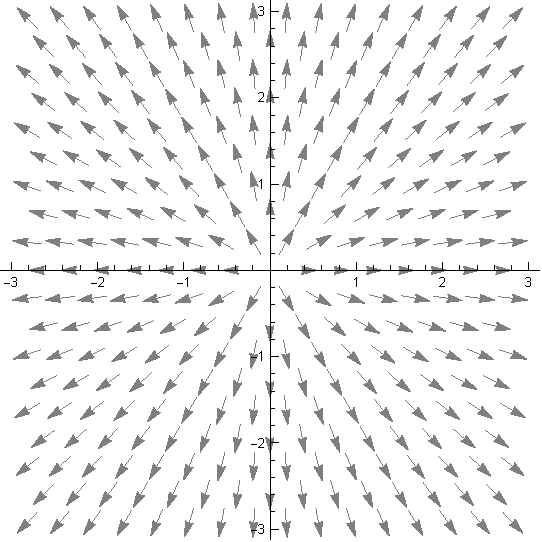
\includegraphics[width=10cm]{images/xyz_vector_field.pdf}
  \end{center}
  Notice that, in terms of spherical coordinates, $\mathbf{F}\left(x,y,z\right) = r\hat{r} = \mathbf{r}$.
\end{example}
\begin{definition}[Incompressible Fluid]
  A fluid is incompressible if its density is constant.\newline

  In particular, incompressible fluids cannot have either sources or sinks, since sources imply a local reduction in density, while sinks imply a local increase in density.
\end{definition}
\begin{example}
  Consider a sprinkler with $N$ streams. Since water is incompressible, the density of streamlines $\sigma$ and the surface area of the spherical shells, $A$ must be inversely proportional to each other.
  \begin{center}
    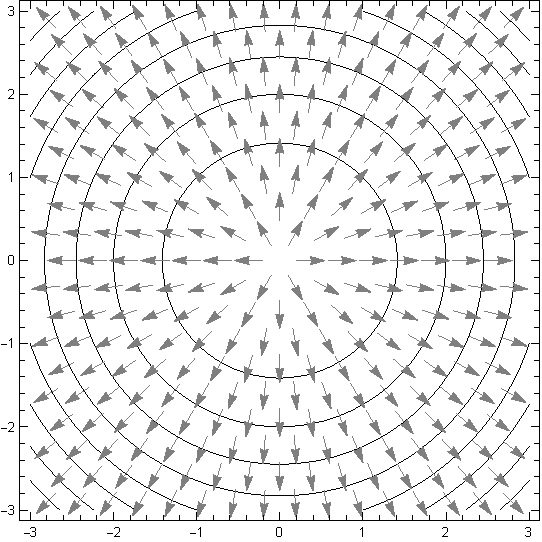
\includegraphics[width=10cm]{images/shells_vector_field.pdf}
  \end{center}
  Thus, we have
  \begin{align*}
    N &=\sigma A,
  \end{align*}
  meaning $\sigma \sim \frac{1}{r^2}$ since $A\sim r^2$.\newline

  In particular, the strength of the vector field must diminish with the square of the distance.
  \begin{center}
    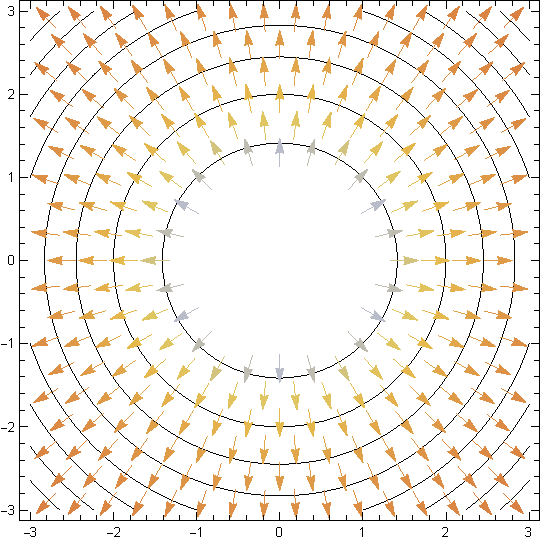
\includegraphics[width=10cm]{images/shells_vector_field_2.pdf}
  \end{center}
\end{example}
\begin{example}
  Vector fields can be added.
  \begin{center}
    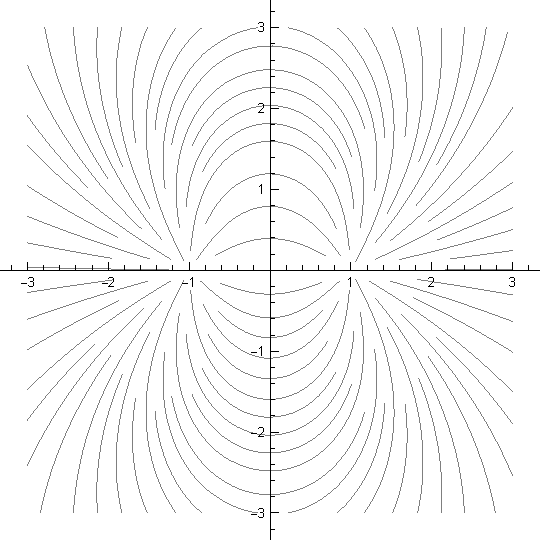
\includegraphics[width=10cm]{images/dipoles.pdf}
  \end{center}
\end{example}
\begin{example}
  Consider the field
  \begin{align*}
    \mathbf{G}\left(x,y\right) &= \frac{1}{\sqrt{x^2 + y^2}}\left(-y\hat{i} + x\hat{j}\right)
  \end{align*}
  As depicted, we can see that the vector field looks as follows.
  \begin{center}
    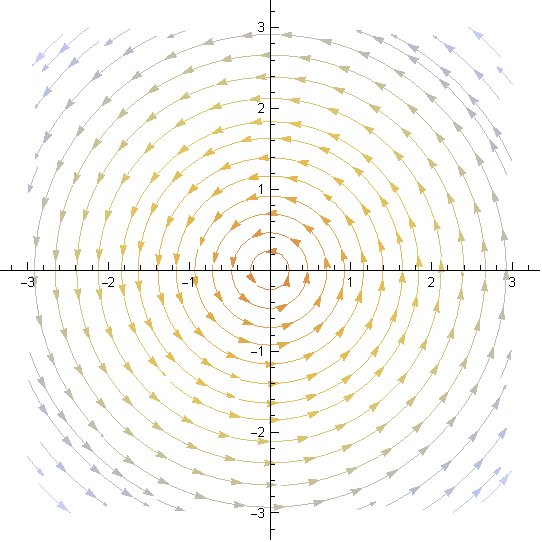
\includegraphics[width=10cm]{images/phihat_field.pdf}
  \end{center}
  In particular, we can see that $\mathbf{G} = \hat{\phi}$.
\end{example}
Notice that our vector fields are dependent on both the basis and the coordinate system.\newline

In particular, we have reason to prefer a Cartesian basis over the polar or spherical basis, since the Cartesian basis is position-independent.
\subsection{Gradient, Divergence, and Curl}%
\begin{center}
  \renewcommand{\arraystretch}{1.5}
  \begin{tabular}{c|c|c}
    Value & Expression In Terms of $\nabla$ & Expression In Terms of $\partial$\\
    \hline
    Gradient & $\nabla f$ & $\pd{f}{x} \hat{i} + \pd{f}{y}\hat{j} + \pd{f}{z}\hat{k}$\\
    Divergence & $\nabla \cdot \mathbf{E}$ & $\sum_{i}\partial_i E_i$\\
    Curl & $\nabla \times \mathbf{B}$ & $\sum_{i,j,k}\epsilon_{ijk}\partial_{i}B_j\hat{e}_k$\\
    Laplacian of a scalar field & $\nabla^2 f$ & $\sum_{i}\frac{\partial^2}{\partial i^2}f$\\
    Laplacian of a vector field & $\nabla^2\mathbf{v}$ & $\sum_{i}\pd{^2}{i^2}v_i \hat{e}_i$
  \end{tabular}
\end{center}
\subsubsection{The $\nabla$ Operator}%

Consider a scalar function $f\left(\mathbf{r}\right)$. If we want to imagine how $f$ changes as we move $\mathbf{r}$ to $\mathbf{r} + d\mathbf{r}$, we use the chain rule.
\begin{align*}
  df &= \left(\pd{f}{x}\right)dx + \left(\pd{f}{y}\right)dy + \left(\pd{f}{z}\right)dz\\
     &= \begin{pmatrix}\frac{\partial f}{\partial x}\\\frac{\partial f}{\partial y}\\\frac{\partial f}{\partial z}\end{pmatrix} \begin{pmatrix}dx\\dy\\dz\end{pmatrix}\\
     &= \nabla f \cdot d\mathbf{r}.
\end{align*}
In particular, we define
\begin{align*}
  \nabla f &= \pd{f}{x} \hat{i} + \pd{f}{y}\hat{j} + \pd{f}{z}\hat{k}.
\end{align*}
Notice that, since $dx\hat{i} + dy\hat{j} + dz\hat{k}$ is a vector, and $df$ is a scalar, we know that $\nabla f$ \textit{must} be a vector.
\begin{definition}[Gradient]
  \begin{align*}
    \nabla f &= \pd{f}{x} \hat{i} + \pd{f}{y}\hat{j} + \pd{f}{z}\hat{k}\\
    df &= \left\vert \nabla f \right\vert \left\vert d\mathbf{r} \right\vert \cos\theta.
  \end{align*}
\end{definition}
If $\nabla f$ is in the direction of $d\mathbf{r}$, then $\cos\theta = 1$, meaning $df$ is maximized. In particular, $\nabla f$ points in the direction of maximum change in $f$.\newline

In particular, this means that for every (differentiable) scalar field, there is a natural vector field associated with the direction of largest increase.
\begin{example}
  The electric field
  \begin{align*}
    \mathbf{E} &= -\nabla V.
  \end{align*}
  Similarly, for any given potential $U$, 
  \begin{align*}
    \mathbf{F} &= -\nabla U.
  \end{align*}
\end{example}
\begin{definition}[The $\nabla$ Operator]
  \begin{align*}
    \nabla f &= \begin{pmatrix}\pd{f}{x}\\\pd{f}{y}\\\pd{f}{z}\end{pmatrix}\\
             &= \underbrace{\begin{pmatrix}\pd{}{x}\\\pd{}{y}\\\pd{}{z}\end{pmatrix}}_{\nabla} \left(f\right)
  \end{align*}
  Thus, we get
  \begin{align*}
    \nabla \equiv \pd{}{x}\hat{i} + \pd{}{y}\hat{j} + \pd{}{z}\hat{k}.
  \end{align*}
\end{definition}
\begin{example}\hfill
  \begin{enumerate}[(1)]
    \item For some scalar field $f\left(\mathbf{r}\right)$, we can take
      \begin{align*}
        \nabla\left(f\right) &= \nabla f,
      \end{align*}
      which yields the gradient field.
    \item For some vector field $\mathbf{E}$, we can take
      \begin{align*}
        \nabla \cdot \mathbf{E} = g
      \end{align*}
      which yields a scalar field known as the divergence of $\mathbf{E}$.\newline

      In particular,
      \begin{align*}
        \nabla \cdot \mathbf{E} &= \pd{}{x}\left(\mathbf{E}\cdot \hat{i}\right) + \pd{}{y}\left(\mathbf{E}\cdot \hat{j}\right) + \pd{}{z}\left(\mathbf{E}\cdot \hat{k}\right).
      \end{align*}
    \item For some vector field $\mathbf{B}$, we can take
      \begin{align*}
        \nabla \times \mathbf{B} = \mathbf{A},
      \end{align*}
      which yields a vector field known as the curl of $\mathbf{B}$.
    \item 
      \begin{align*}
        \nabla \cdot \left(\nabla f\right) &= \left(\nabla \cdot \nabla\right) f\\
                                           &= \pd{^2 f}{x^2} + \pd{^2 f}{y^2} + \pd{^2 f}{z^2}\\
                                           &= \nabla^2 f\\
                                          &= \Delta f,
      \end{align*}
      which yields an operator known as the Laplacian.
  \end{enumerate}
\end{example}
\begin{example}
  Let $\mathbf{v}_1 = xy\hat{i} + y^2\hat{j}$. Then,
  \begin{align*}
    \nabla \cdot \mathbf{v}_1 &= \pd{}{x}\left(xy\right) + \pd{}{y}\left(y^2\right)\\
                              &= y + 2y\\
                              &= 3y,
                              \intertext{and}
    \nabla \times \mathbf{v}_1 &= \left(\pd{}{x}\left(y^2\right) - \pd{}{y}\left(xy\right)\right)\hat{k}\\
                               &= -x\hat{k}.
  \end{align*}
\end{example}
\begin{example}
  Let $\mathbf{v}_2 = \frac{1}{x^2 + y^2 + z^2}\left(x\hat{i} + y\hat{j} + z\hat{k}\right)$. Then,
  \begin{align*}
    \nabla \cdot \mathbf{v}_2 &= \pd{}{x}\left(\frac{x}{x^2 + y^2 + z^2}\right) + \pd{}{y}\left(\frac{y}{x^2 + y^2 + z^2}\right) + \pd{}{z}\left(\frac{z}{x^2 + y^2 + z^2}\right)\\
                              &= \frac{1}{x^2 + y^2 + z^2}
    \nabla \times \mathbf{v}_2 &= 0
  \end{align*}
\end{example}
\begin{example}
  Consider
  \begin{align*}
    \mathbf{v} &= x^2 \hat{i} + y^2 \hat{j} + z^2\hat{k}\\
    \mathbf{u} &= yz\hat{i} + zx\hat{j} + xy\hat{k}.
  \end{align*}
  In particular, it is easily verified that $\nabla \times \mathbf{v} = 0$ and $\nabla \cdot \mathbf{u} = 0$.
\end{example}
\subsubsection{Applying Vector Identities to the $\nabla$ Operator}%
We are aware that
\begin{align*}
  a\mathbf{V} &= \mathbf{V}a\\
  \mathbf{A}\cdot \mathbf{B} &= \mathbf{B}\cdot \mathbf{A}.
\end{align*}
However, when we deal with $\nabla$, we have to respect both the properties of the vectors \textit{and} the properties of the operator. In particular,
\begin{align*}
  f\nabla \neq \nabla f.
\end{align*}
This is because $f\nabla$ is a vector operator, while $\nabla f$ is a vector field. Similarly,
\begin{align*}
  \nabla \cdot \mathbf{E} \neq \mathbf{E}\cdot \nabla,
\end{align*}
since $\nabla \cdot \mathbf{E}$ is a scalar field, while $\mathbf{E}\cdot \nabla$ is a scalar operator.
\begin{example}[Curl of Curl]
  Consider
  \begin{align*}
    \nabla \times \left(\nabla \times \mathbf{v}\right).
  \end{align*}
  On first glance, we want to use the identity $\mathbf{A}\times \left(\mathbf{B}\times \mathbf{C}\right) = \mathbf{B}\left(\mathbf{A}\cdot \mathbf{C}\right) - \mathbf{C}\left(\mathbf{A}\times \mathbf{B}\right)$, yielding
  \begin{align*}
    \nabla \times \left(\nabla \times \mathbf{v}\right) &= \nabla\left(\nabla \cdot \mathbf{v}\right) - \mathbf{v}\left(\nabla \cdot \nabla\right).
  \end{align*}
  However, notice that $\mathbf{v}\left(\nabla \cdot \nabla\right)$ is a scalar operator, while $\nabla \times \left(\nabla \times \mathbf{v}\right)$ is a vector field. Thus, we have to modify the double cross product to $\mathbf{A}\times \left(\mathbf{B}\times \mathbf{C}\right) = \mathbf{B}\left(\mathbf{A}\cdot \mathbf{C}\right) - \left(\mathbf{A}\times \mathbf{B}\right)\mathbf{C}$
  \begin{align*}
    \nabla \times \left(\nabla \times \mathbf{v}\right) &= \nabla\left(\nabla \times \mathbf{v}\right) - \nabla^2 \mathbf{v}.
  \end{align*}
\end{example}
\begin{example}[Curl of Gradient and Divergence of Curl]
  Consider
  \begin{align*}
    \nabla \times \left(\nabla f\right).
  \end{align*}
  In particular, we are tempted to take
  \begin{align*}
    \nabla \times \left(\nabla f\right) &= \left(\nabla \times \nabla\right)f\\
                                        &= 0.
  \end{align*}
  This is allowed, since we do not affect the property of the operation.\newline

  The following identity is also true,
  \begin{align*}
    \nabla \cdot \left(\nabla times \mathbf{v}\right) &= 0,
  \end{align*}
  but we cannot use a cheesy method to prove this.
\end{example}
\begin{remark}
  Faraday's law is $\nabla \times \mathbf{E} = 0$, and Gauss's law for magnetism is $\nabla \times \mathbf{B} = 0$, where $\mathbf{E}$ denotes the electric field and $\mathbf{B}$ denotes the magnetic field.\newline

  If $\nabla \times \mathbf{E} = 0$ in electrostatics, then $\mathbf{E} = \nabla A$ for some scalar function $A$. In particular, we say $\mathbf{E} = -\nabla V$. We call $V$ the scalar potential.\newline

  Similarly, if $\nabla \cdot \mathbf{B} = 0$, then $\mathbf{B} = \nabla \times \mathbf{A}$ for some vector field $\mathbf{A}$. We call $\mathbf{A}$ the vector potential.
\end{remark}
\begin{example}[Products]
  Consider
  \begin{align*}
    \nabla \left(fg\right).
  \end{align*}
  Using the product rule, we have
  \begin{align*}
    \nabla \left(fg\right) &= \left(\nabla f\right)g + f\left(\nabla g\right).
  \end{align*}
  However, when we look at
  \begin{align*}
    \nabla \cdot \left(f\mathbf{A}\right),
  \end{align*}
  things get a little more complicated. Notice that $\nabla \cdot \left(f\mathbf{A}\right)$ is a scalar, meaning we apply the product rule using dot products to yield such a scalar.
  \begin{align*}
    \nabla \cdot \left(f\mathbf{A}\right) &= \nabla f \cdot \mathbf{A}  + f\nabla\cdot \mathbf{A}.
  \end{align*}
  Similarly,
  \begin{align*}
    \nabla \times \left(\mathbf{A}f\right) &= \left(\nabla \times \mathbf{A}\right)f + \nabla f \times \mathbf{A}\\
                                           &= \left(\nabla \times \mathbf{A}\right)f - \mathbf{A}\times \nabla f.
  \end{align*}
\end{example}
\subsubsection{Changing Coordinates}%
Vector equations are fundamentally independent of their coordinate systems. Thus, the established identities in the previous subsection must be valid regardless of the coordinate system.\newline

For instance, we should be able to calculate
\begin{align*}
  \nabla \cdot \mathbf{E}
\end{align*}
regardless of the coordinate system.
\begin{example}[Converting to Polar Coordinates]
  Consider
  \begin{align*}
    \mathbf{v}_1 &= xy\hat{i} + y^2\hat{j}.
  \end{align*}
  Conversion to polar coordinates yields
  \begin{align*}
    \mathbf{v}_1 &= \left(r^2\sin\phi\right) \hat{r}.
  \end{align*}
\end{example}
\end{document}
